% ---------------------------------------------------------------------
%                      DOCUMENTO DE EJEMPLO
%                    DE TFG/TFM DE LA ETSII
% ---------------------------------------------------------------------

\documentclass[tfm, rm, english]{tfgtfmetsii}
\usepackage[titletoc]{appendix}
\usepackage[backref=true]{biblatex}
\usepackage[colorlinks=false]{hyperref}
\usepackage{cleveref}
\usepackage{multicol}
\usepackage{mathrsfs}
%\hypersetup{
 %   colorlinks=true,
  %  linkcolor=blue,
   % filecolor=magenta,      
    %urlcolor=cyan,
%}
 
%\urlstyle{same}


%\usepackage[pagebackref]{hyperref}
%\usepackage[hyperpageref]{backref}
%\usepackage[colorlinks]{hyperref}
%\hypersetup{pdffitwindow=true,linkcolor=LightSkyBlue,citecolor=Sienna,urlcolor=Navy,menucolor=black}
%\usepackage[hyperpageref]{backref}

\makeatletter
\@addtoreset{chapter}{part}
\makeatother
% Opciones de la clase 'editorialupv'
%
% tfg         - TFG
% tfm         - TFM
% rm          - Tipo de letra roman
% sf          - Tipo de letra sanserif
% nomathskip  - No se modifican las distancias de las ecuaciones 
%
% castellano  - La publicaci�n est� escrita en castellano
% valencia    - La publicaci� est� escrita en valenci�
% english     - La publicaci�n est� escrita en ingl�s

% T�tulo del TFG


\newcommand{\TFGtitulo}{Este es el t�tulo del TFG}

% T�tulo del TFM

\newcommand{\TFMtitulo}{Automatic representation of the electrical grid layout}

% ---------------------------------------------------------------------
% Configuraciones presonalizadas 

% ---------------------------------------------------------------------
% ---------------------------------------------------------------------
% Configuraci�n general

\usepackage{inputenc}
\usepackage[T1]{fontenc}

\ifcastellano\usepackage[spanish,es-tabla]{babel}\fi
\ifvalencia\usepackage[catalan]{babel}\fi
\ifenglish\usepackage[english]{babel}\usepackage{csquotes}\fi
\newcommand{\sen}{\on{sen}}	


\usepackage{xcolor}
\usepackage{array,booktabs}
\usepackage{tabularx,longtable,multicol}
\usepackage{amssymb}

%\ifenglish
%	\raggedright % No justifica, i no divide las palabras con guiones
%\fi

% ---------------------------------------------------------------------
% ---------------------------------------------------------------------
% Bibliograf�a

\usepackage[
	url = false,
	style = authoryear,
	hyperref = true,
	backref = true,
	backend = biber, % Otra opci�n es 'backend = bibtex'
	backend = bibtex,
	]{biblatex}

% ---------------------------------------------------------------------
% ---------------------------------------------------------------------
% Documento electr�nico

\usepackage{makeidx}
\makeindex


\colorlet{colorEnlace}{black} 


\usepackage[
	{colorlinks},
	{linkcolor=colorEnlace},
	{citecolor=colorEnlace},
	{urlcolor=colorEnlace},
	{bookmarksnumbered},
	{breaklinks},
	]{hyperref}

% ---------------------------------------------------------------------
% ---------------------------------------------------------------------
% Expresi�n de unidades seg�n el Sistema Internacional, monedas

\usepackage{eurosym}
\usepackage{siunitx}

\ifenglish
	\sisetup{output-decimal-marker={.}}
\else
	\sisetup{output-decimal-marker={,}}
\fi

\DeclareSIUnit[number-unit-product = {\;}] \EURO{\geneuro}

% ---------------------------------------------------------------------
% ---------------------------------------------------------------------
% Comandos y entornos personalizados


% ---------------------------------------------------------------------

\newcommand{\ingles}[1]{\textit{#1}}

% ------------------------------------------------------------------------

\usepackage{xspace}

\newcommand{\angles}[1]{\textit{#1}\/}
\newcommand{\miUrl}[1]{{\small%
	%\texttt%
	{\underline{#1}}}}

\newcommand{\matlabr}{{\sc Matlab}$^\circledR$\xspace}
\newcommand{\simulinkr}{\textit{Simulink}$^\circledR$\xspace}
\newcommand{\matlab}{{\textsc{Matlab}}\xspace}
\newcommand{\simulink}{\textit{Simulink}\xspace}

\newcommand{\scr}{\textit{script\/}\xspace}
\newcommand{\scrs}{\textit{scripts\/}\xspace}

% ------------------------------------------------------------------------

\definecolor{griset}{rgb}{.925, .925, .925}

	\newsavebox{\mybox}
	\newenvironment{parrafoDestacado}
		{%
		\fboxsep = 2ex
		\fboxrule = .4pt
	  	\begin{lrbox}{\mybox}%
	  	\begin{minipage}{.85\textwidth-2\fboxsep}\itshape\parskip=2ex
		}
		{%
		\end{minipage}
	  	\end{lrbox}%
		\begin{flushright}
			\colorbox{griset}{\usebox{\mybox}}%
	  		%\fcolorbox{black}{griset}{\usebox{\mybox}}%
		\end{flushright}
		}
		
%	\newenvironment{parrafoDestacado} % Si no nos gusta el sombreado
%		{
%		\vspace{0ex}
%		\begin{quote}\noindent
%		\itshape
%		\samepage
%		\parskip=2ex
%		%\color{NavyBlue}
%		}
%		{
%		\end{quote}
%		}



% ------------------------------------------------------------------------
% Resumen del cap�tulo


	\newsavebox{\myboxb}
	\newenvironment{Resumen}
		{%
		\vspace*{-2.0cm}
		\fboxsep = 0pt
		\fboxrule = 0pt
	  	\begin{lrbox}{\myboxb}%
	  	\begin{minipage}{.85\textwidth}\itshape\parskip=2ex\parindent=2em
		}
		{%
		\end{minipage}
	  	\end{lrbox}%
		\begin{flushright}
			\usebox{\myboxb}%
		\end{flushright}
		\vspace{0.5cm}
		}



% ---------------------------------------------------------------------
% ---------------------------------------------------------------------
% S�mbolos matem�ticos

\newcommand{\on}{\operatorname}

% ---------------------------------------------------------------------
% ---------------------------------------------------------------------
% Teoremas y ejemplos

\ifcastellano
	\newtheorem{teorema}{\upshape\bfseries Teorema}[section]
	\newtheorem{lema}{\mdseries\scshape Lema}[section]
	\newtheorem{proposicion}{\upshape\bfseries Proposici�n}[section]
	\newtheorem{ejemplo}{\bfseries\scshape Ejemplo}[section]
\fi

\ifvalencia % Es mantenen els mateixos noms per compatibilitat, per� l'autor els pot personalitzar
	\newtheorem{teorema}{\upshape\bfseries Teorema}[section]
	\newtheorem{lema}{\mdseries\scshape Lema}[section]
	\newtheorem{proposicion}{\upshape\bfseries Proposici�}[section]
	\newtheorem{ejemplo}{\bfseries\scshape Exemple}[section]
\fi

\ifenglish
	\newtheorem{teorema}{\upshape\bfseries Theorem}[section]
	\newtheorem{lema}{\mdseries\scshape Lemma}[section]
	\newtheorem{proposicion}{\upshape\bfseries Proposition}[section]
	\newtheorem{ejemplo}{\bfseries\scshape Example}[section]
\fi



% ---------------------------------------------------------------------



\addbibresource{referencias.bib}
\bibliography{referencias}
%\bibliographystyle{unsrt}
\DefineBibliographyStrings{english}{%
    backrefpage  = {see p.}, % for single page number
    backrefpages = {see pp.} % for multiple page numbers
}



% ---------------------------------------------------------------------
% Las carpetas para los gr�ficos

\graphicspath{
	{./figuras/}
	{./logos/}
	}

% ---------------------------------------------------------------------

\title{
	Automatic representation of the electrical grid layout\\
	Manual de uso de la plantilla para \LaTeX\ de \TF{}s de la ETSII\\[3ex]
	\mdseries\large	Enero de 2017
	}

\author{
	Jorge Arpa Garzaran
}

% ---------------------------------------------------------------------
% ---------------------------------------------------------------------
% ---------------------------------------------------------------------
% ---------------------------------------------------------------------


\newcommand{\PartialToc}{\hrule\vspace*{1pc}%
\startcontents[Chapter]\vbox{\bfseries\Large Overview}
\printcontents[Chapter]{}{1}{}\vspace*{1pc}\hrule}


\begin{document}



% ---------------------------------------------------------------------
% Referencias cruzadas personalizadas y texto autom�tico de LaTeX

\ifcastellano % Las definiciones predefinidas empiezan con may�scula
	\renewcommand{\itemautorefname}{punto}
	\renewcommand{\sectionautorefname}{seccin}
	\renewcommand{\subsectionautorefname}{subseccin}
	\renewcommand{\subsubsectionautorefname}{subseccin}
	\renewcommand{\figureautorefname}{figura}
	\renewcommand{\tableautorefname}{tabla}
	
	\renewcommand{\indexname}{ndice alfabico}
	\renewcommand{\bibname}{Bibliograf}
	\renewcommand{\contentsname}{dice general}
	\renewcommand{\abstractname}{Resumen}	
\fi

\ifvalencia % �s molt important fer aquestes definicions, si no, apareixeran en angl�s
	\renewcommand{\itemautorefname}{punt}
	\renewcommand{\sectionautorefname}{secci}
	\renewcommand{\subsectionautorefname}{subsecci}
	\renewcommand{\subsubsectionautorefname}{subsecci}
	\renewcommand{\figureautorefname}{figura}
	\renewcommand{\tableautorefname}{taula}

	\renewcommand{\indexname}{dex alfabtic}
	\renewcommand{\bibname}{Bibliografia}
	\renewcommand{\contentsname}{dex}
	\renewcommand{\abstractname}{Resum}	
\fi

% -------------------------------------------------------

\frontmatter

% -------------------------------------------------------
% P�gina de t�tulo

%\maketitle	



\chapter{Portada del \TF}


La portada del \TF es un elemento NORMALIZADO, y la no utilizacion de la portada normalizada puede suponer motivo de no aceptacion de la solicitud de defensa.

La portada normalizada es un pdf que esta disponible en la web de la ETSII: 

\texttt{\enlacedescargas}

se sugiere que tras rellenarlo sea impreso en PDF y adjuntado al PDF de esta memoria.




% -------------------------------------------------------
% Resumen, pr�logo o prefacio

\cleardoublepage
\phantomsection

\addcontentsline{toc}{chapter}{\abstractname}
\setcounter{tocdepth}{3}



\chapter{Declaration} 


This dissertation is the result of my own work and contains nothing but my personal work  as part of the HERGE team, except where specified in the text and in \nameref{Acknowledgements}. It is to be presented before both \ingles{Universidad Politecnica de Valencia}'s and \ingles{Ecole Centrale Marseille}'s juries, respectively as Master's thesis and \ingles{Travail Fin d'Etudes} of the double degree there pursued, while nevertheless ensuring RTE confidentiality requirements are respected.

I hereby declare that except where specific reference is made to the work of others, the contents of this dissertation are original and have not been submitted in whole or in part for consideration for any other degree of qualification in this, or any other university, but those above referred.
This dissertation contains fewer than 65.000 words including appendices, bibliography, footnotes, tables and equations and has fewer than 150 figures.

 \begin{flushright}
 
\Author
\\
\Date
\end{flushright}


% ---------------------------------------------------------------------
% ---------------------------------------------------------------------

\chapter*{\abstractname}

% ---------------------------------------------------------------------
% ---------------------------------------------------------------------
\ifcastellano

Este es un documento de ejemplo en el que se utiliza la plantilla para redactar \TF{}s con \LaTeX\ para la ETSII de la Universitat Politca de Vaia. Esta plantilla la puedes descargar en la siguiente direccin web:

% Pendiente de cambiar por la web de la ETSII
{\small\href
	{http://www.upv.es/entidades/AEUPV/info/Plantilla_LaTeX_UPV_2016.zip}
	{\url{http://www.upv.es/entidades/AEUPV/info/Plantilla_LaTeX_UPV_2016.zip}}}

En el \hyperref[sec:Manual]{primer caplo} encontrar un manual de uso de la plantilla, en el que te indicamos los pasos que debes seguir y las recomendaciones para aplicar satisfactoriamente la plantilla a tu documento. 

Por otro lado, en el \autoref{cap:recomendaciones} se recogen las recomendaciones de redacci estilo para el desarrollo del Trabajo Fin de Grado/Men la ETSII.

Esperamos que te sea este documento de ejemplo, y el manual que contiene. Te agradeceremos que nos envs cualquier sugerencia o error que detectes en la plantilla.

\fi

\ifvalencia

Este es un documento de ejemplo en el que se utiliza la plantilla para redactar \TF{}s con \LaTeX\ para la ETSII de la Universitat Polita de Vaa. Esta plantilla la puedes descargar en la siguiente dir


% Pendiente de cambiar por la web de la ETSII
{\small\href
	{http://www.upv.es/entidades/AEUPV/info/Plantilla_LaTeX_UPV_2016.zip}
	{\url{http://www.upv.es/entidades/AEUPV/info/Plantilla_LaTeX_UPV_2016.zip}}}

En el \hyperref[sec:Manual]{primer captulo} encontrars un manual de uso de la plantilla, en el que te indicamos los pasos que debes seguir y las recomendaciones para aplicar satisfactoriamente la plantilla a tu documento. Adems, se recogen las recomendaciones de redacc y estilo para el desarrollo del Trabajo Fin de Grado en la ETSII.

Este resumen es el que apareceen el repositorio de la UPV cuando cualquier persona acceda a consultar este documento. Por ello debe recoger de forma concisa y precisa el contenido, alcance y resultados obtenidos. Su e 300 palabras. 

Esperamos que te seaeste documento de ejemplo, y el manual que contiene. Te agradeceremos que nos ecualquier sugerencia o error que detectes en la plantilla.

\fi

\ifenglish

The impetus of this thesis was documenting the improvements implemented during my Final Master's internship.

This primer builds on common concepts, such as or 

 \TF{}s con \LaTeX\ para la ETSII de la Universitat P Esta plantilla la puedes descargar en la siguienten web:

% Pendiente de cambiar por la web de la ETSII
{\small\href
	{http://www.upv.es/entidades/AEUPV/info/Plantilla_LaTeX_UPV_2016.zip}
	{\url{http://www.upv.es/entidades/AEUPV/info/Plantilla_LaTeX_UPV_2016.zip}}}

En el \hyperref[sec:Manual]{primer caplo} encontrar un manual de uso de la plantilla, en el que te indicamos los pasos que debes seguir y las recomendaciones para aplicar satisfactoriamente la plantilla a tu documento. Ades, se recogen las recomendaciones de redac y estilo para el desarrollo del Trabajo Fin de Grado en la ETSII.

Esperamos que te seatil este documento de ejemplo, y el manual que contiene. Te agradeceremos que nos enes cualquier sugerencia o error que detectes en la plantilla.

\fi


%\vfill


\begin{center}
	\begin{tabular}{c@{\hspace{1.5cm}}c}
		Jorge Arpa Garzaran
		& 
		
		
		Jean-Etienne Lemaire
		\\
		\href{mailto:jarpagarzara@centrale-marseille.fr}{\small jarpargarzara@centrale-marseille.fr}
		&
		
		
		\href{mailto:jean-etienne.lemaire@rte-france.com}{\small jean-etienne.lemaire@rte-france.com}
	\end{tabular}
\end{center}

\ifcastellano

\textbf{Palabras Clave:} Incluir las palabras clave del \TF

\fi

\ifvalencia

\textbf{Paraules clau:} Incloure les paraules clau del \TF
\fi

\ifenglish

\textbf{Keywords: BIG DATA, layout, Wiring diagram, Electrical layout, FME, ESMI} 

\fi

% ---------------------------------------------------------------------





\chapter{Acknowledgements} \label{Acknowledgements}

\begin{parrafoDestacado}
"First of all, I would like to acknowledge my two tutors: \texttt{Jean Etienne Lemaire} and \texttt{Philippe Rapin}, for the aid displayed, their proximity and all the advice given throughout these last 6 months. I am convinced it has certainly enriched and will channel my future professional steps in the experiences yet to come.
Thanks also to \texttt{Heng Ngeth} for his constant availability and proximity towards my integration within the work group."
\end{parrafoDestacado}

En el caso de que se desee puede dedicarse una pina para agradecimientos. El formato de agradecimientos es libre siempre que se mantenga el tipo de letra definido como base del formato. Por ello se admiten agradecimientos del estilo: 

\begin{parrafoDestacado}
``Quiero aprovechar la ocasi para agradecer el apoyo de mis ... y de mis ...  Asimismo no puedo olvidar en este momento a mis comperos ...''
\end{parrafoDestacado}

Aunque tambin se admiten agradecimientos de la forma: 

\begin{flushright}
`` A mi familia\linebreak 
   A mi tutor  \linebreak
   A mis comperos \linebreak
... ''
\end{flushright}

\chapter{Acronyms}
\label{Acronyms}

\textbf{Subscript - poner en varias columnas??}
\begin{longtable}{@{} >{}p{0.18\textwidth} @{\hspace{0.05\textwidth}} p{0.8\textwidth} @{}}
    \textit{Cellule}
    &
    Bay\\
    
    \textit{Disjoncteur}
    &
    Breaker\\
    
    \textit{Jeu de barres}
    &
    BusbarSection\\
    
    \textit{Liaison intrasite}
    &
    ACLineSegment\\
    
    \textit{Poste}
    &
    VoltageLevel\\
    
    \textit{Terminal}
    &
    Terminal\\
    
    \textit{Sectionneur d'aiguillage}
    &
    Disconnector\\
    
    \textit{Transformateur}
    &
    PowerTransformer\\
    
\end{longtable}

\textbf{Abbreviations}

\begin{longtable}{@{} >{\ttfamily}p{0.1\textwidth} @{\hspace{0.13\textwidth}} p{0.85\textwidth} @{}}

	AIG
	&
	Automatic Image Generation\\
	
	AML
	&
	Automatic Machine Learning\\
	
	API
	&
	Application Program Interface\\
	
	APOGEE
	&
	\ingles{Anticipation du Poste Opératuer Pour une Gestion Evoluée du système Electrique}\\
	
	BPMF
	&
	Business Process Model and and Notation\\
	
	CAD
	&
	Computer-Aided Design\\
	
	CDL
	&
	CIM Diagram Layout\\
	
	CIM
	&
	Common Information Model\\
	
	CSV
	&
	Comma Separated Values\\
	
	DPOSE
	&
	\ingles{Département Programmes Outil du Sytème Electrique}\\
	
	DSIT
	&
	\ingles{Direction des Systèmes d'Information et des Télécomunications}\\
	
	EMF
	&
	Eclipse Modeling Framework\\
	
	EMS
	&
	Energy Management System\\
	
	EPRI
	&
	Electrical Power Research Institute\\
	
	ESRI
	&
	Environmental System Research Institute\\
	
	ETL
	&
	Extract Transform Load\\
	
	FoS
	&
	Field of Study\\
	
	FME
	&
	Feature Manipulation Engine\\
	
	GAME
	&
	\ingles{Gestion Anticipée et Maitrise de l'Exploitation}\\
	
	GIS
	&
	Geographical Information Systems\\
	
	HERGE
	&
	\ingles{"RG" - Réferentiel Graphique}\\
	
	HV
	&
	High Voltage\\
	
	IEEE
	&
	Insitute of Electrical and Electronics Engineers\\
	
	IEC
	&
	International Electrotechnical Commission\\
	
	ITESLA
	&
	
	\\
	
	MDS
	&
	Multidimensional Scaling\\
	
	MDA
	&
	Model Driven Architecture\\
	
	MEP
	&
	\ingles{Mise en Production}\\
	
	MV
	&
	Medium Voltage\\
	
	NERC
	&
	North American Electric Reliability Council\\
	
	OSCAR
	&
	\ingles{Outil de Saisie des Contrats d'Accès au Réseau}\\
	
	PANDA
	&
	\ingles{Portail d'Appui tactile et Numérique du DispAtcher}\\
	
	POC
	&
	Proof Of Concept\\
	
	PoV
	&
	Point of View\\
	
	RDF
	&
	Resource Description Framework\\
	
	SCADA
	&
	Supervision Control And Data Acquisition\\
	
	SID
	&
	\ingles{Système d'Information Décisionnel}\\
	
	SNC
	&
	\ingles{Système National de Conduite}\\
	
	SRC
	&
	\ingles{Système Reginal de Conduite}\\
	
	TSO
	&
	Transmission System Operator\\
	
	UML
	&
	Unified Modeling Language\\
	
	VM
	&
	Virtual Machine\\
	
	XML
	&
	Extensible Markup Language\\
	
	nomathskip  
	& 
	Si no se deja un linea entre las ecuaciones destacadas y los p�rrafos anterior y 
	siguiente, debes activar esta opci�n, \autoref{sec:manual:matematicas}.\\
	 

\end{longtable}




% -------------------------------------------------------
% �ndice: tabla de contenidos


\cleardoublepage
\phantomsection

%\addcontentsline{toc}{chapter}{\contentsname}
%\setcounter{tocdepth}{2}
%\addcontentsline{toc}{subsection}{\subsectionsname}%{\arabic{chapter.\arabic{section}.\arabic{subsection}}

\tableofcontents
\listoffigures
\listoftables

% -------------------------------------------------------
% Numeraci�n de p�ginas n�meros ar�bicos
% Primer cap�tulo en p�gina 1

\mainmatter

% -------------------------------------------------------
% -------------------------------------------------------
% -------------------------------------------------------
% Estructura en partes del TFG/TFM

%\part{Memory}


% Cap�tulos de la memoria

\chapter[Introduction]{Introduction}
\label{cap:Intro}

\begin{Resumen}

This first chapter aims on giving the reader a panoramic overview of the problematic of study, raising consciousness on the work carried out through an introspective day-to-day approach PoV. Thus, the existing \nameref{sec:Intro:framework}\footnote{Projet HERGE was the teamwork in which my \ingles{stage} was framed, will be explained in detail in the section \ref{sec:Intro:thesis-purpose:HERGE}} is firstly stated, altogether with a \nameref{sec:intro:thesis-purpose:background} and a \nameref{sec:Intro:thesis-purpose} introduction, subsequently enriched in \hyperref[sec:Intro:Thesis-purpose:Outcomes]{management} and \hyperref[sec:Intro:Thesis-purpose-Budget]{financial} terms.

\end{Resumen}
\PartialToc
% ---------------------------------------------------------------------
% ---------------------------------------------------------------------

\bigskip
\lettrine[lines=2]{\textbf{A}}{}utomatization in any FoS, and neatly regarding image generation (AIG) has been markedly spread around multiples domains over the last decade, to the extend that it is presently being used for any kind of technology without us necessarily noticing out. Its threshold and applications vary from those most puristic ones, usually linked to the Artificial Intelligence (AI) branch (with a vast bibliography published on tackling human eye AIG recognition behaviour\footnote{The way in which humans systematically identify an object can be assessed and analyzed from the AIG's PoV} \cite{Eyevision}, annotation and description \cite{Automaticimageannotation,Automaticdescgeneration}, or semantic association \cite{Naturallanguage} in images generation processes), to those focused on a more pragmatic approach in Machine Learning (ML): developping genetic algorithms \cite{Genetic_algorithms}, image to text deep learning\footnote{Half-way between computer vision, natural language processing and AI, deep learning has been extensively used for sites, posts and, roughly, for any element of representation labeling} \cite{Deep_learning_image_to_text}, or software diagrams \cite{Software_diagrams} automatically.

Anyhow, a vast range of methodological algorithms for image generation of one-line diagrams have been successfully implemented in recent years \cite{Distribution-feeder,standard-based-SLD-AG,AlgoAIG}. Such being the case of our object of study, its practical use strictly based on a corporate database source, deeply suggested an integrated data treatment process. Hence the interest of \href{https://www.safe.com/how-it-works/}{Feature Manipulation Engine (FME)} usage, a powerful tool fed on web-sources, application and any kind of data roughly speaking, which, via its conglomeration and the enhancement on logically-linked image displaying thanks to \href{http://www.esri.com/}{Environmental Systems Research Institute (ESRI)} - \nameref{sec:approach:software:ArcGIS} technologies, has finally resulted on a rigorous, edge-cutting, still intuitive corporate tool. 

With this aim, a methodogical process for automatic Rte's network diagram representation is proposed on this work. Remarkably, the latter being completely adaptable to corporate patrimonial databases while being performed on departmental  tools, as those previously stated. 
% ---------------------------------------------------------------------
\section{Framework}
\label{sec:Intro:framework}

My final-degree internship project has been pursued as part of HERGE, which governed by GAME - \ingles{Gestion Anticipée et Maitrise de l'Exploitation} - team, constitutes all at once an important part of DPOSE - \textit{Département Programmes et Outiles du Système Electrique} - dept. All those, contained in the DSIT - \ingles{Direction Systèmes d'Information et Télecom} - dept., constitute the latent force of Rte - \ingles{Réseau Transport d'Electricité}'s technical solutions development. 

Two tutors (\texttt{Jean-Etienne Lemaire} in a first 3-months time-lap, and \texttt{Philippe Rapin} in the coming three) have encompassed my activity in the context of HERGE, with the constant assistance of \texttt{Heng Ngeth} in technical and bureaucratical matters. 
Henceforth, all these elements will be concreted in detail from a macroscopic to a technically tangible horizon going over the stages from the \hyperref[sec:Intro:Rte]{entreprise} scope, to the \hyperref[sec:Intro:thesis-purpose:HERGE]{project in question's}: 


\subsection{Rte}
\label{sec:Intro:Rte}

Rte is born in 2000 as a result of \href{https://eur-lex.europa.eu/eli/dir/1996/92/oj}{\texttt{European Directive No. 96/92/EC of December 1996}} aiming to completely keep generation and transmission national companies independent. Four years later, Rte's activities completely unbundled EdF's - \textit{Electricité de France} - and therefore their divestiture finally becomes a reality, granting its trademark rights from them on.

The sole Transmission System Operator (TSO) in metropolitan and continental France plays a strategic role that goes way beyond the implicit meaning of the term "power transmission" gatewaying geneartors, industirial consumers MV distributors, rail companies and market traders  activity.

\begin{figure}[h!]
    \centering
    \parbox[t]{0.6\textwidth}{
    {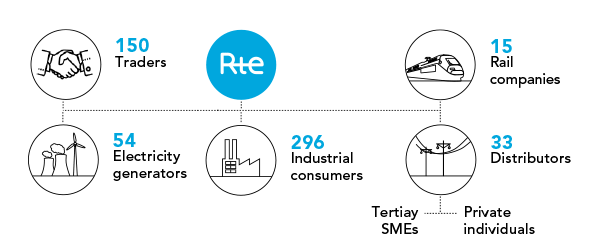
\includegraphics[width=0.6\textwidth]{0.figuras/clients.png}}
    \captionof{figure}{Rte clients portfolio.}}
    \label{fig:Rte-portfolio}
\end{figure}

Within a strictly-regulated framework supplying grid access in completely fair competition, as overseen by the Energy Regulatory Commission (CRE), Rte balances its grid round-the-clock, while broadening its ressources of tomorrow in order to \textit{"ensure security of supply and sustainable electricity system operation, to guarantee the same quality of service for everybody, to continually improve our services, and to contribute to the economic development of the territories"} (citing expressly from the corporate webpage).

With nearly 105,000 km of lines, RTE has eversince canalized the national and international financial activity through the biggest grid in whole Europe: 46.2 \% of which extra-high voltaged lines (400 and 225 kV\footnote{Regional sub-transmission is performed at 150, 90 and 63 kV}), which rout annually about 495 TWh\footnote{Annual energy transit flow remains virtually steady over the last years \cite{IEC-normative}.} all over the hexagon and \href[https://www.rte-france.com/sites/default/files/2015_05_20_flow_based_brochure.pdf]{beyond}, where reaching 112 TWh thanks to 60 cross-border connections with neighbouring countries.

\begin{figure}[ht]
    \centering
    \parbox[t]{0.475\textwidth}{
    \centering
    {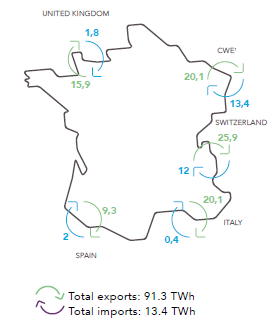
\includegraphics[width=0.475\textwidth]{0.figuras/exports-imports.png}}
    \captionof{figure}{International exports-imports flux.}
    \label{fig:Rte-portfolio}
    }
    \hfill
    \parbox[t]{0.475\textwidth}{
    \centering
    {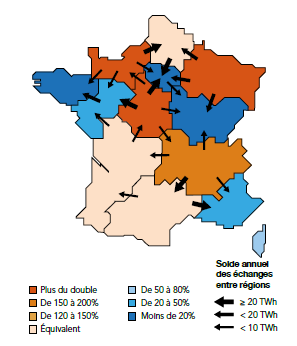
\includegraphics[width=0.475\textwidth]{0.figuras/prod-consumption-national.png}}
    \captionof{figure}{National flux exchanges between regions in 2015.}
    \label{fig:National-exchangues}
    }
\end{figure}



Its employees continuous training program empowers its mainstay: e.g. the versatile knowledge and visibility of its high-skilled 8,279 employees-officials workforce, responsibles of the exploitaton and maintenance of 1,231 transformers, 2,710 substations and 3,504 delivery points, whose rate of burying between 2014 and 2015 reached a 97 \%.

RTE, with an actual turnover of €4,126 million in 2007, and yielding a profit of €466 million\footnote{Both up slightly from previous year, which RTE attributed to increases in network access payments and interconnector capacity auctions revenues.}, has constantly endeavoured to offer its customers safe, economic and clean access to electrical power. There is no shortage of projects: extension of market coupling to Southern European countries, installation of smart substations, using drones to maintain infrastructures...
%REVISAR ULTIMO PARRAFO

%ANADIR IMAGNES GRAFICOS LOGO??	

\subsection{DPOSE}
\label{subsec:Intro:thesis-purpose:DPOSE}

Hierarchical continent of HERGE, DPOSE conforms the Rte's tool development dept., as its literally labelling translation\footnote{Electric Systems tools \& software Dept.} stands for. And its actual functionalities do not differ much from that: formed by a team of engineers highly trained in software development and abstract thinking, HERGE feeds Rte with a vast range of software conception, development and, finally, industrial production launch. Branched in 5 big subsections, and grouping about 100 employees, they are as follows:

%HABLAR CON GUILLAUME PARA CADA UNA DE ESTAS RAMAS

%FORMATO DE LA TABLA QUE TENIA ANTES
%{
%\setlength{\extrawaheight}{2ex}

%\begin{longtable}{@{} >{\ttfamily}p{0.1\textwidth} @{\hspace{0.01\textwidth}} p{0.85\textwidth} @{}}
\begin{description}


\item{\textbf{GAME -} \ingles{Logiciels DV} - Software DV.} GAME frames the whole dept.'s activity, by proposing technical solutions in terms of applications and human-machine interface (HMI) \ingles{Mise en production} (MEP), that is, projects channelling from their conception to the final industrialization launching.
 \\

\item{\textbf{OSCAR (\ingles{Outil de Saisie des Contrats d'Accès au Réseau}) - }\ingles{Management en temps réel} - Real-time management.}   It is responsible of ensuring project continuity exploitation in the real time, making solutions animated by other departments physically possible and therefore to make them become a reality. Neatly, it manages the different clients' portfolio automatic access to the electrical network.\\

\item{\textbf{SID (\ingles{Système d'Information Décisionnel}) - }\ingles{Héberger} - Host.} In charge of the inter-applications info management, by fire-walling its flow through telecommuted devices.\\

\item{\textbf{StanWay - }\ingles{Conduire} - Carry}. The future communications tool. It is destined to replace SRC and SNC actual system in all the exploitation centres.\\

\item{\textbf{STEP (\ingles{Systéme Téleconduite Et Passarelle}) - }\ingles{Configurer} - Configure.} Data management tool. It encompasses the different \texttt{steps} information takes.\\

\end{description}
%\end{longtable}

\begin{figure}[h!]
    \centering
    \parbox[t]{0.6\textwidth}{
    {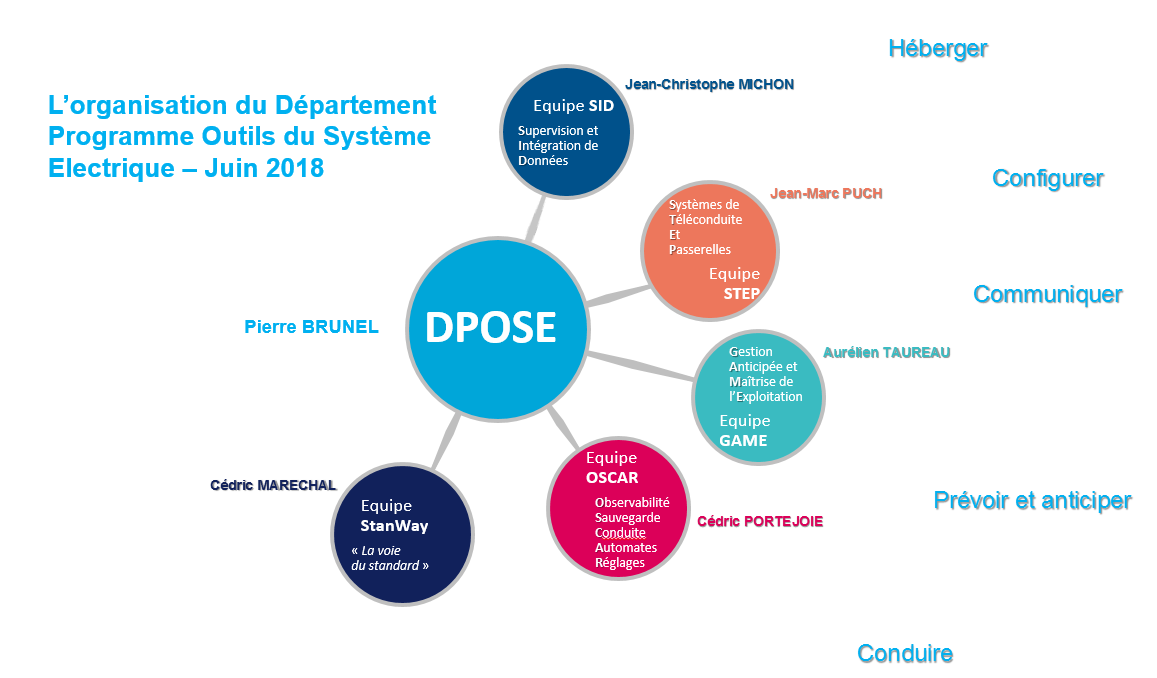
\includegraphics[width=0.6\textwidth]{0.figuras/DPOSE.png}}
    \captionof{figure}{Projects hierarchical interdependences within DPOSE.}}
    \label{fig:DPOSE}
\end{figure}

\subsection{HERGE}
\label{sec:Intro:thesis-purpose:HERGE}

Framed around a 5-person team and leaded by my tutor Jean-Etienne Lemaire, whose functions were retaken in early August by Philippe Rapin, HERGE consists of a mulitidsciplinary high-formed team of engineers, aimed to create an intutive and interactive interface of the french HV\footnote{Henceforth we will consider \texttt{High Voltage, } for tensions from 63 to 400 kV, commonly designed as the \texttt{Transport phase}.} and eventually MV\footnote{We will consider \texttt{Medium Voltage}, for tensions from 4 to 63 kV, commonly designed as the \texttt{Distribution phase}} electrical network, discredited in 7 regional zones represenation, plus a national one.
Framing the project in the tools-developping section for Operation Management anticipation (DPOSE), it consists of an ambitious project focused on three key activities:
\begin{itemize}
    \item \textbf{Represent} graphically the network and its subconstituents unequivocally and perennially over time.
    \item\textbf{Provide} all the corporate SRC and SNC users with a unique and lisible network layout representation, enabling its perfect contextualization.
    \item \textbf{Normalize} network representation for the Exploitation Dept. at any time horizon.
\end{itemize}

\begin{figure}[h]
    \centering
    \parbox[t]{1\textwidth}{
    \href{https://herge-portal.rte-france.com/arcgis/apps/webappviewer/index.html?id=84a7af442f014844bd95939ce3c0067a}{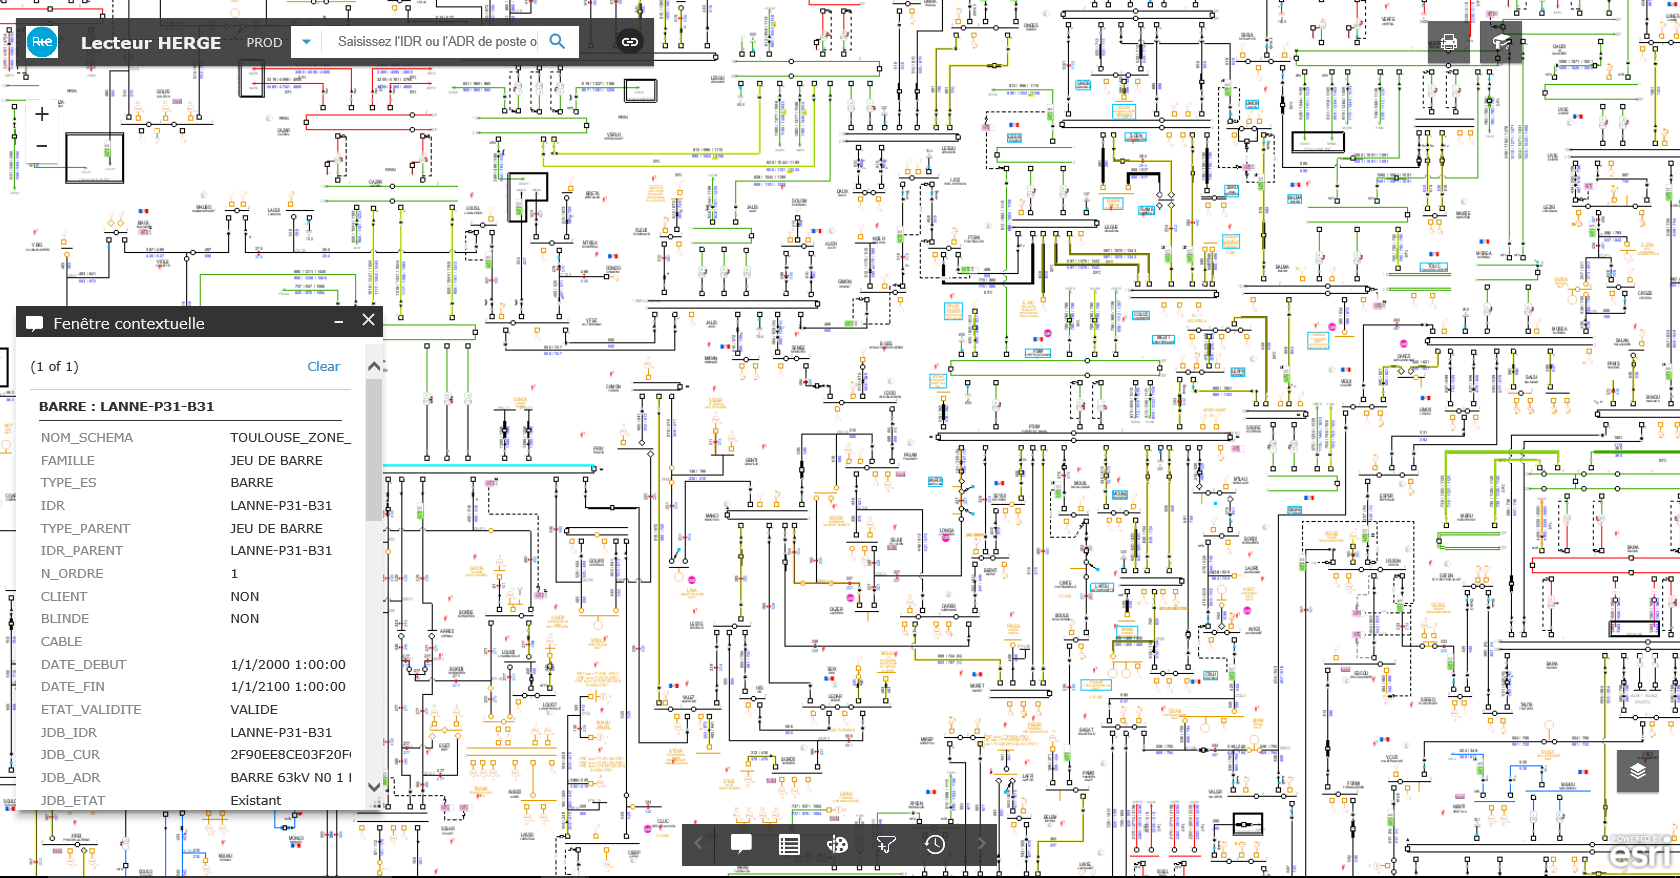
\includegraphics[width=1\textwidth]{0.figuras/HERGE_interface.png}}
    \captionof{figure}{HERGE interface layout. Click on the image to acces RTE's electrical diagram layout interface}}
    \label{fig:herge}
\end{figure}

%QUITAR IMAGEN ORGANIZACION OPERATIVA DSIT

%\begin{figure}[h]
   % \centering
    %\parbox[t]{1\textwidth}{
    %\href{}{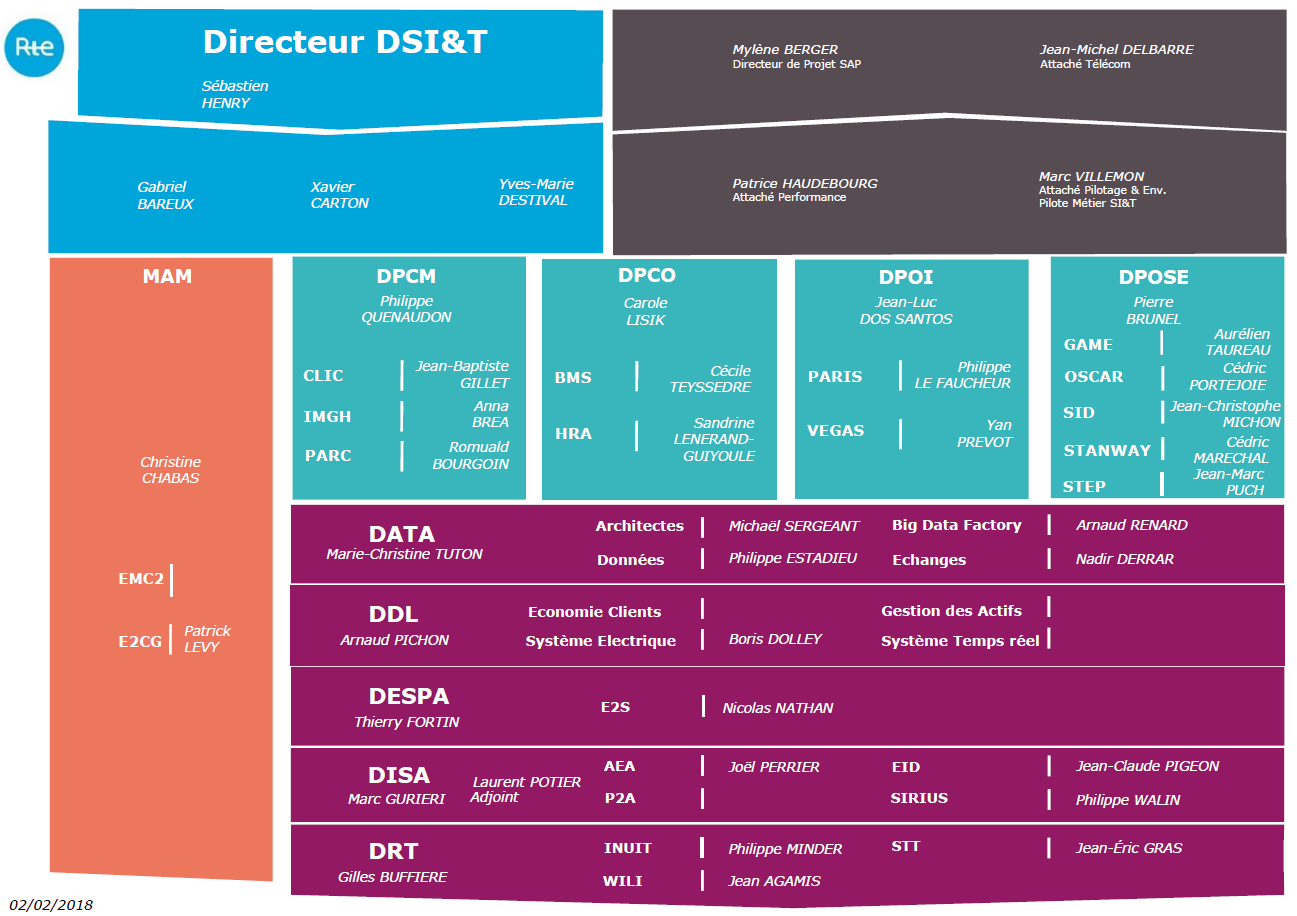
\includegraphics[width=1\textwidth]{0.figuras/DSIT_organization_chart.png}}
    %\captionof{figure}{DSIT organizational chart. HERGE is contained in GAME Dept., under the lead of Aurélien Taureau.}}
    %\label{fig:dsit}
%\end{figure}

%UNIR CADA UNA DE LAS ZONAS A UN PLANO EN ANEXOS???

HERGE is therefore responsible of displaying the electric diagram layout for the 7 zones (\ingles{CNES Quart, Lille, Lyon, Marseille, Nancy, Nantes, SQY Po and Toulouse}) where SRC has been discretised. Henceforward, HERGE will enrich the former electric diagram with a voltage colour coding, plus  elements ordering control possibilities, thus giving birth to \nameref{cap:AIG} of Herge. 

As defined in its corporate culture, RTE's employees are not expected to remain in a certain post for more than 4 year. This fact boosts the common collective feeling and enlarges the competences field of all workers. Furthermore, it turns  documentation into a vital tool for ensuring continuity of the projects, which frequently exceed its members' stay. 

Additionally, HERGE's specifications expect it to become a real-time version, and may have very interesting potential application in the foreseeable future. Specifically, it seeks to provide the dispatcher with a tactile interface, intended to make its layout interpretation easier, clearer and therefore much more efficient. Therefore a first step towards HERGE's amortization has been bureaucratically already materialized. Not only this fonctionallity will embrace its old functions, but will also step forward as a referent for other projects feeding, with consequent inter-projects iterations for everyone's tender specifications meeting. Neatly, regarding StanWay's influence, conversations have already begun and exchanges between projects are more common, and more appropiate.

\subsubsection{Corporate framework}
\label{subsubsec:Intro:thesis-purpose:Framework:corporate-framework}
Framed in a multidimensional environment, the present project impacted and was impacted by a wide spectrum of factors of all kinds, which are explained with detail in the following.
The usage of independent layouts, even throughout a same enterprise is widely spread among Rte's non-concomitant projects. Each of them are displayed according to different basis, and it's under this non-uniqueness representation model that underlie many of the daily problems in a daily HERGE's employee day-to-day life. It is on this basis that several inter-departmental  meetings were hold between members of the teams STANWAY and APOGEE in order to enrich mutual knowledge and approaching of a mutual problem, and standardize thereafter an unique representation criteria, noting projects' aims diverged considerably seldom.

In addition, HERGE responsibilities and application diverge from a wide range of projets and departments, and therein resides the fundamental difficulty of the problem. Hereafter, a full list of the potential daily HERGE users is displayed. 

\begin{itemize}
    \item\textbf{Operation Management Dept.-} \ingles{Service Conduite} - 293 employees: in charge of the weekly updating, corresponding to the instant t.
    
    \item\textbf{Planning Management Dept. -} \ingles{Service Planification} - 151 employees: in charge of the network evolution. Using network schemes for incoming activities planning.
    
    \item\textbf{Strategy Dept. -} \ingles{Service Strategy} - 99 employees.
    
    \item\textbf{Performance Dept. -} \ingles{Service Performance} - 58 employees.
    
    \item\textbf{Maintenance Dept.}
    
    \item\textbf{Research \& Developpement Dept. -} \ingles{Développement et Ingénierie}.
    
    
\end{itemize}


All those stakeholders, potentially impacted by the numerous approach changes undertaken, constitute a big part of the enterprise activities. Whatsoever, by the moment of my arrival, Herge's approach was completely alien to StanWay's, hoping it is not that much by the moment I leave the project, the following actions have been taken. 

In particular, all the stakeholders were contacted and put together in order to overcome with the optimal solution for the inital purpose of alleviating this objectives' misalignment, leading to a considerable consciousness-raising of the bureaucratic side within such a multilateral-concerned project. Decisions were taken with mutual consent and efforts were mainstreamed in the pursuit of every part's best, contributing all this to ramp up the intern's skill and integration within the work-group.

\begin{description}

	\item\textbf{Herge}: DPOSE-branched subsection, it aims on an interactive web interface realization. Further information has been provided in the section \ref{sec:Intro:thesis-purpose:HERGE}, with an aim in deeper \ingles{raison d'être} explanation and specific roles detailing.

	\item\textbf{StanWay}: also DPOSE-branched, it is a project in charge of the new corporative SCADA deploiement. SCADA (Supervision Control And Data Acquisition) is a \textit{"control system architercture that uses computers, networked data communications and graphical user interfaces for high-level process supervisory management"} (Wikipedia).
	
	\item\textbf{Itesla}:  Research and Development (R\&D) Dept. - branched, independent from DPOSE's continent, e.g. DSIT (\ingles{Direction des Systèmes d'Ingénierie et Télecom)}, and in charge of the former SCADA deployment, it puts together a various and numerous set of teams, working altogether for the RTE of tomorrow.
	
	\item\textbf{Convergence}: Moreover, than a departement, it represents a deeply-shared tool that makes the reformating and interexchangue of the multiple format types possible. It boosts therfore the continuity of all kind of problems, even if their approaches may diverge considerably at first sight. 
	
	\item\textbf{Apogee}: ITESLA-branched, they display real-time breaker changes due to operator decision and/or unexpected events. Their Java-sourced approach is consistently different, but the target and delivrables stay pretty close to HERGE's, and relatively interchangable via CONVERGENCE's archive reformatting. Indeed, they delivred .iidm files as their doc outcome.
	
\end{description}

Anyway, Rte departamental structure consitute a knowledge network  Multidimensional knowledge sharing between all these projects has been vital for profitable evolutions in a participatory way, thanks to Rte's proactive philosophy underlying.

\subsubsection{Educational framework}
\label{subsubsec:Intro:Thesis-purpose:Framework:Educational-framework}

In educational terms, this documents constitutes at once several independent livrables, framed all them in the pursuit of my studies. It will firstly be my Master in Industrial Engineering's Thesis, as \ingles{Trabajo Final de Grado}\footnote{Master's Thesis equivalent in Spanish educational regulatory framework} of a 4-plus-2 years Bachelor's \& Master's degree program in the \ingles{Universidad Politécnica de Valencia}. At the same time, this document represents the \ingles{Travail de Fin d'Etudes} of \ingles{Ecole Centrale Marseille}'s studies i.e. a 3-year academical course final thesis, as a part of a Double Master simultaneously there pursued.
All at once, it gathers all the procedure undertaken during a 6-month internship as \ingles{Stage de Fin d'Eudues}, for which this documents constitutes its \ingles{Rapport de stage}\footnote{End of Studies internship's report in French educational regulatory framework.}.

%Tambi�n encontrar�s un archivo denominado `\texttt{preambulo.tex}', donde hemos incluido algunas configuraciones y macros personalizables. Puedes aprovechar este archivo para cargar los paquetes adicionales que utilices en tu publicaci�n.

% ---------------------------------------------------------------------
\section{Thesis purpose}
\label{sec:Intro:thesis-purpose}

The final goal of this Master Thesis's lies on the automatizing of Rte's electrical layout diagram, as a part of the HERGE projet. The team had already an interface prototype running, completely functional and performing, but in which elements dispositions had been previously handmade in AutoCAD by an architect, and no-automatizing was displayed, apart from certain elements labeling.

Numerous stakeholders were affected and interested by this corporate challenge and that influenced considerably the project scope and so did it its approaching too. It was finally those stakeholders who both will afterwards get use of the app outcome and had financed its implementation.

% ---------------------------------------------------------------------

\subsection{Background and \ingles{état de l'art}}
\label{sec:intro:thesis-purpose:background}

Nowadays, the major issue before research and energy industry is the mounting uncertainty that complicates financial viability of the major investments required for the development of edge-cutting technologies and innovative projects. IoT\footnote{Internet of things, refers to the interconnection of multiple devices to transfer autonomously all kind of data, aiming to shorten physical and digital worlds gaps.}: Block-chains, miners, Artificial Intelligence, 3D-printing are some of the edge-cutting technologies promoting this sudden turnarounds in the last decade, which are "likely to be more dramatic than those undertaken during the last century altogether"\footnote{citing explicitly the book 'How Customer Behaviour and Technology Will Change the Future of Financial Services'.}. Enterprises seem to be increasingly concerned on this matter, and are markedly reshaping their business models and working methods. Nevertheless, the emergence of multiple business domains and the big reticence has boosted startups spread-up.   
Rte, well aware of this reality, is turning its sight into edge-cutting, modern projects, such as Apogee, Stanway, Itesla, etc. Herge is indeed one of those potentially high-impact projects in an environment where lot of potential profit underlies, as shows the wide literature and software deployment in the FoS of any nature of LD's AIG, which traditionally hand-desingned. Worth of special mention is \nameref{sec:Diagram:CIMDesk} software, used by Stanway, and which served us for symptomatic processes correlation. 

\begin{figure}[ht]
    \centering
    \parbox[t]{0.475\textwidth}{
    \centering
    {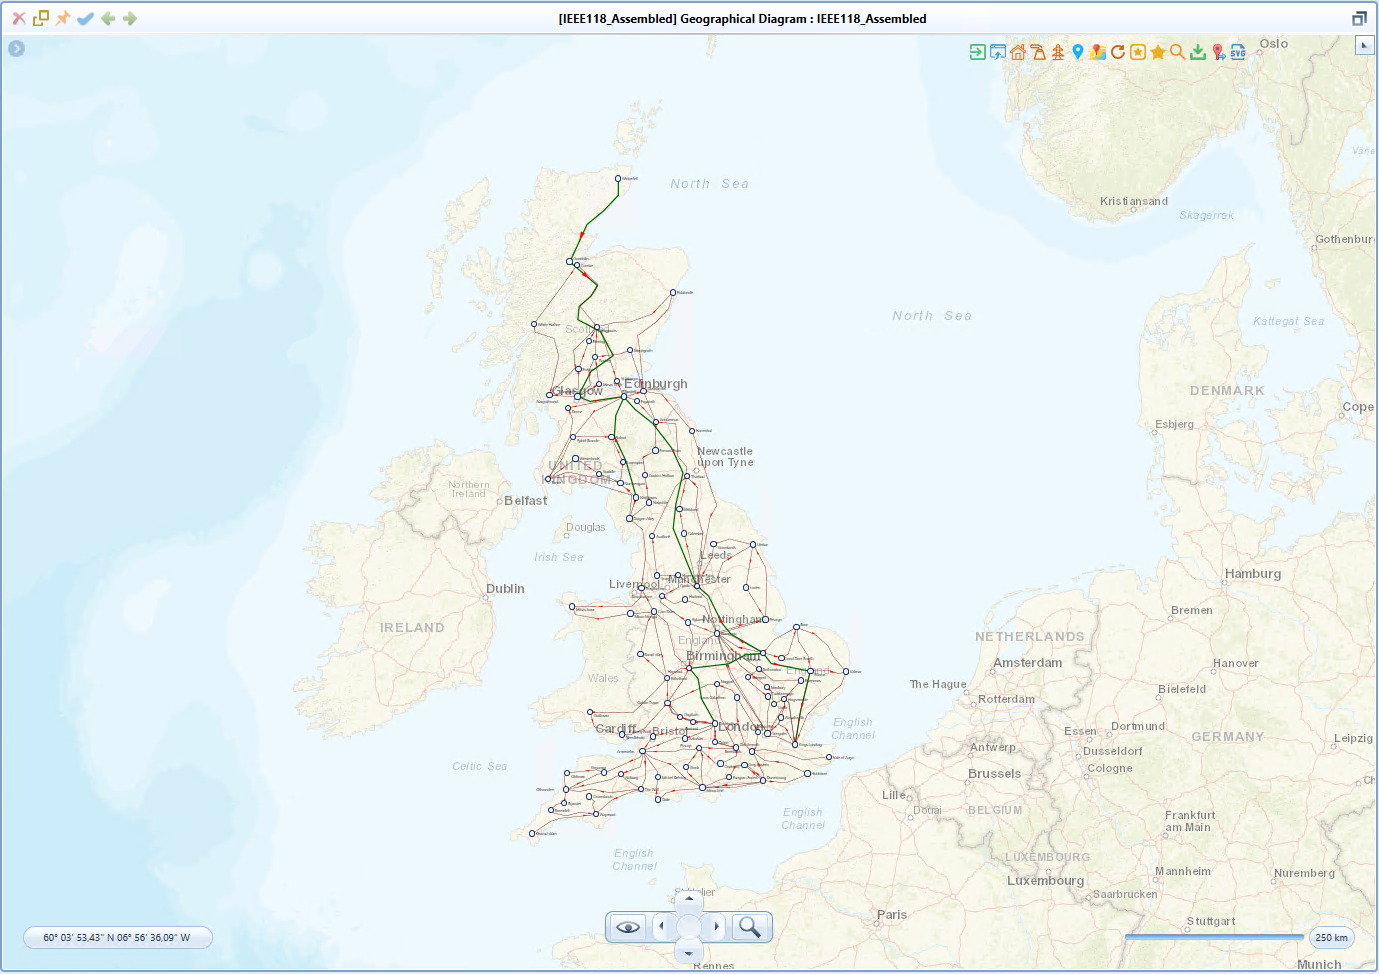
\includegraphics[width=0.475\textwidth]{0.figuras/CIMdesk_england_chart.png}}
    \captionof{figure}{England electric network flux chart displayed with CIM Desk.}
    \label{fig:CIMDesk}
    }
    \hfill
    \parbox[t]{0.475\textwidth}{
    \centering
    {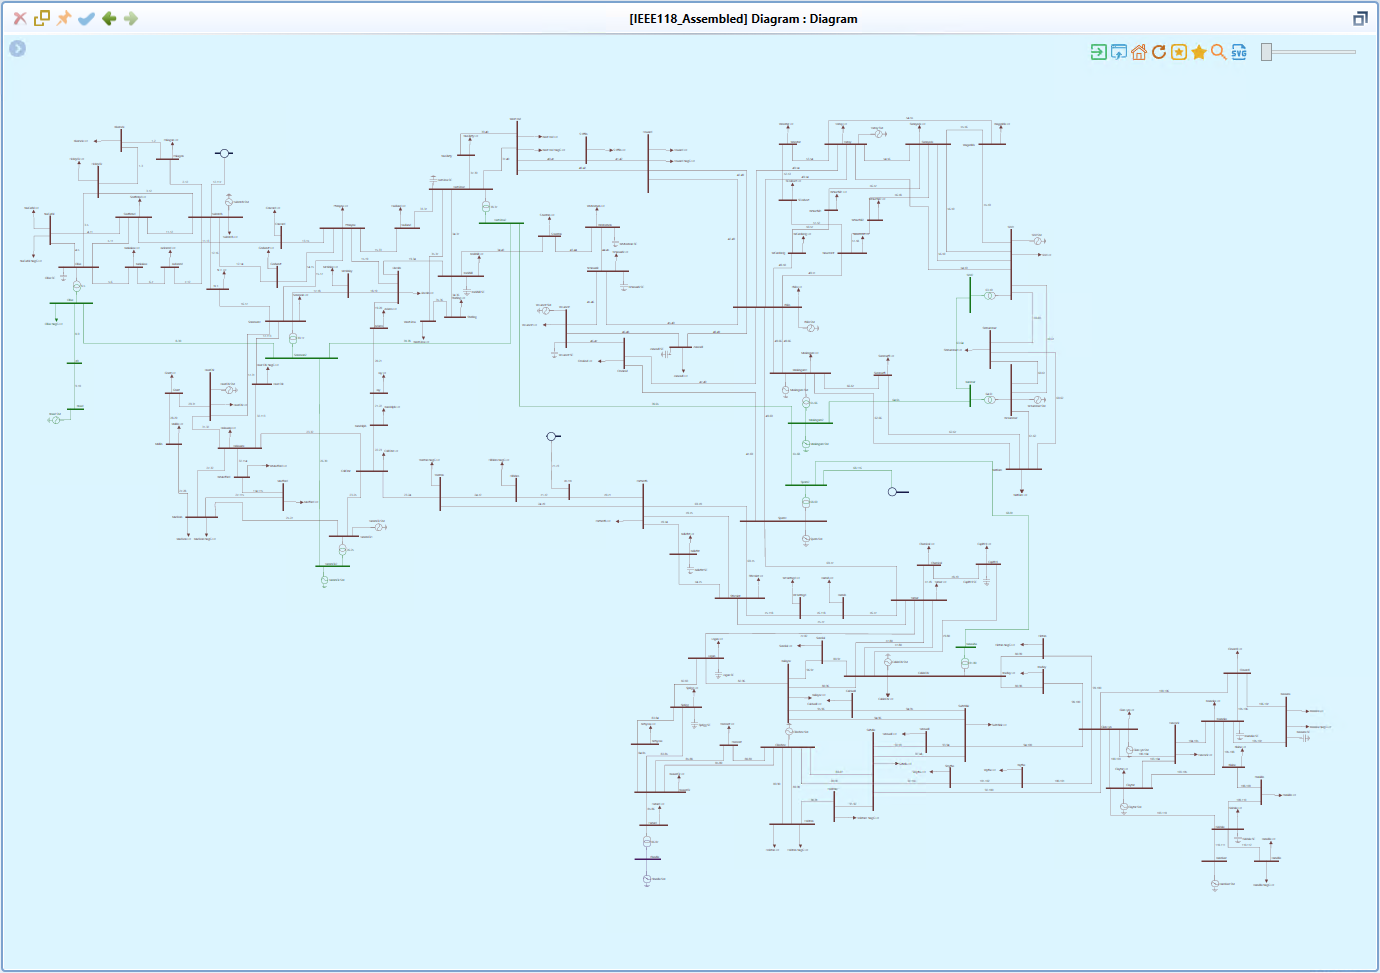
\includegraphics[width=0.475\textwidth]{0.figuras/CIMdesk_england_network_electrical_chart.png}}
    \captionof{figure}{England electric network diagram drawn from its flux chart interpretation with CIM desk.}
    \label{fig:CIMDeskdiagram}
    }
\end{figure}

A vast range of design software exists onto Computer Aided-Design (CAD) of electrical LDs: \textit{See Electrical, DesingSpark Electrical, Bentley's Promis-E, Eplan Electric} or just the \textit{AutoCAD Electrical Toolset} are CAD-based tools that enabled certain automatizing in electrical block components introduction, which finally are to be hand designed by an architect. Thus their automatizing from databases patrimonial remaining certainly unexplored, the necessity of CIM Diagram Layout (CDL) interfaces for streamlining the whole processes is therefore sufficiently substantiated.

Consequently, an skill improvement in XML, RDF and other database formats understanding and contextualizing has been carried out, as seen \hyperref[fig:UMLprofile]{in the following UML class diagram}. To achieve the target goal of network architecture automatizing, deep database usage seems to be the best technically feasible solution in the short term \cite{Automaticdescgeneration, CIMIEE, CIMDistribution}. In addition, and  profiting the corporate patrimony and extensive knowledge of several Rte's employees \cite{specif_detaillees_GAI, IEC-normative, Infos_GAI} of the state of art among the principle european and international distribution companies, a standardized database treatment process was pursuit.

\begin{figure}[h]
    \centering
    \parbox[t]{0.8\textwidth}{
    \centering
    {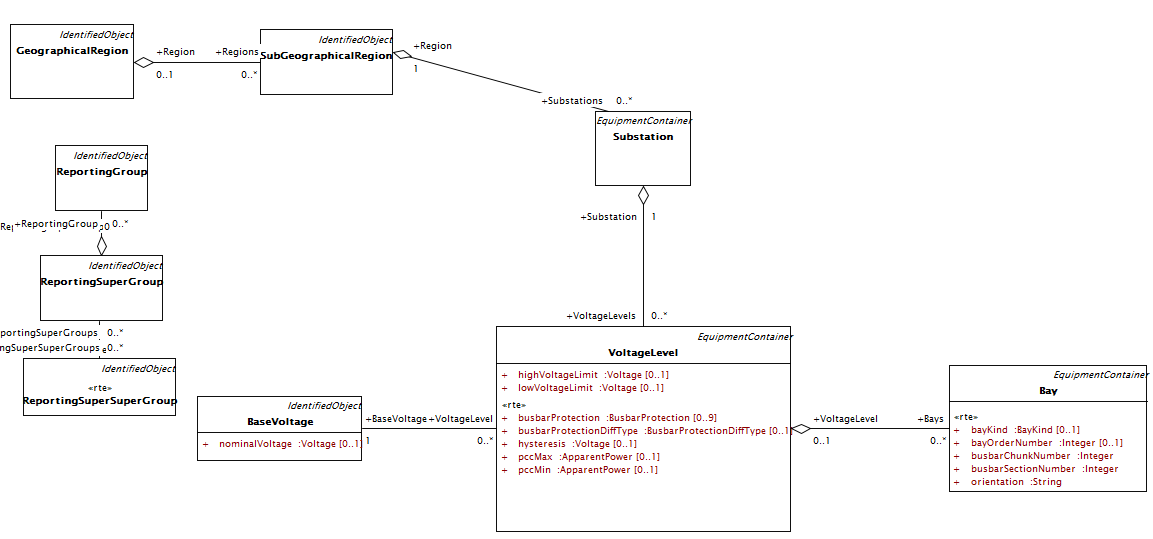
\includegraphics[width=0.8\textwidth]{0.figuras/UML_RTE_geographical_region.png}}
    \caption{UML profile of the substation level dependencies.}
    \label{fig:UMLprofile}}
\end{figure}

Indeed, certain steps have been already taken ahead troughout interesting development studies on the topic, undertaken in SouthKorean \cite{standard-based-SLD-AG} and Indian \cite{Distribution-feeder} research centers. Being the majority of those projects code-oriented \cite{Eyevision, CIMjava}, that is, their deployment sustaining in a low-level language coding implementation, Herge diverges from this approach and comes up with a more intuitive, user-oriented approach. Thus, basically based on the use of \nameref{sec:approach:software:FME}, and relying on corporate patrimonial database refreshment, this software is intended to turn the way AIG of diagram layout have traditionally been designed upside down. 

%%\begin{figure}[h]
    %\centering
    %\parbox[t]{0.8\textwidth}{
    %\centering
    %{\includegraphics[width=0.8\textwidth]{}}
  %%  \captionof{figure}{UML profile of the substation level dependencies.}}
%%    \label{fig:UML_profile}
%%\end{figure}

Some avenues of recourse that could enrich the FME post-treatment have been explored and assessed, mainly \nameref{sec:approach:software:ArcGIS}-linked for post position management for the purpose of a better space usage and interconnection network optimization. Those exploitation routes are deduced from the implementation \nameref{subsub:AIG:SLV:graph_theory}, \nameref{subsub:AIG:SLV:graph_theory:meta_algorithms}, \nameref{subsub:AIG:SLV:Voronoi} or Multidimensional Scaling (\nameref{subsub:AIG:SLV:MDS}) to the problematic of study. All of them are discussed in detail in section \ref{sub:AIG:SLV:theoretical background}.

%INSPIRARSE EN EL ARTICULO SOBRE BOCKCHAIN DE IGNACIO MADRID ENCONTRADO EN LA REVISTA SMART GRIDS INFO QUE HE GUARDADO EN MARCADORES

% ---------------------------------------------------------------------
\subsection{Project approach}
\label{sec:introduction:thesis-purpose:project-approach}

Constituting the graphical interface for the most part of Rte's on-field business users, an important flux of financial actives depend on Herge's fate, which makes it a substantially constrained project in terms of users necessities. They are the ones who grab the major part of the negotiating power and therefore who encompass the trail of the project.

Consequently, the results of the displayed methodology shall remain certainly close to the actuals, and changes may be considerably evident, flexible and easily apprehensible. This incertitude reigning all the project long has deeply impacted its approach and methodology, always on the pursuit of flexibility by means of modularity and adaptability possibilities in connection to the future additional steps Herge could take, yet as all its impacted partners.

Apart from the technical approach, a managerial PoV was assessed all along the project, as it remained absolutely non static and deeply impacted by the approach during certain evolution phases. For this reason and overall on the skill ramp-up periods, several meeting were held with the automatic network representation mainstream corporate voices on the matter for a proper state of art drafting, and the different technical solutions to address sketching.

In this purpose, \hyperref[subsub:introduction:thesis-purpose:project-approach:parties]{several ateliers and meetings} have been arranged specially on the ferirst stage of the internship for boosting a correct sill ramp up altogether with a project contuxtualization.  To confront the incertitude coming from a vast range of inputs, \hyperref[subsub:introduction:thesis-purpose:risk-assessement]{a risk matrix }has been performed at the first stages of the project. It has been nevertheless systematically completed in the face of changes found progressively, and notably after identifying other projects adhesions.


\subsubsection{Concerned parties}
\label{subsub:introduction:thesis-purpose:project-approach:parties}

In this line, numerous stakeholders have been confronted through the project contextualization. Their roles and importance divergence between them, and their interdependence with Herge impacts its actions and viceversa.

The main projets that were contextually confronted to Herge are as follows:
\begin{description}
    \item[- StanWay:]
    One of the biggest projects in Rte at the moment. 35M€-budgeted, it aims to create a huge data exchanging platform, for the different levels of corporate data acquisiton, and, regarding us, for SCADA structure layout deployment.
    \item[- Apogee:]
    Inside the DDL department, it consists on an coding platform, striving for homologous purpose to StanWay's. I.e, energy real-time flux management
    
\end{description}

\subsubsubsection{StanWay}
\label{sec:approach:project-approach:parties:stanway}

The information flux was continuous and considerable between both projects, whereas their approaches and objectives sometimes diverged. Nevertheless, increasing incertitude was present regarding mutual influence of projects. That is, even if SI dept. head aimed at an unique and versatile scheme with rules reflecting both projects interests, fieldwork responsibles expected specific outcomes and preponderant stoicism of HERGE, as its performance, even if it was not too elegant, casted no doubts when applied. It remains in contact touch with the edge-cutting enterprises in the matter for technical complementation assessment: e.g. General Electrics, Siemens, PSI and ABB were assessed, their performacnce results shown in \autoref{fig:Kiviat_StanWay_supp} here below. 

\begin{figure}[h!]
    \centering
    \parbox[t]{0.7\textwidth}{
    \href{}{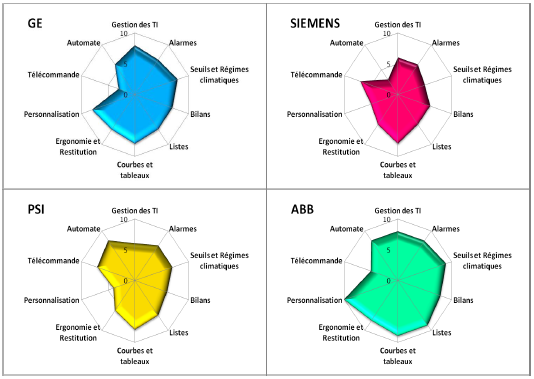
\includegraphics[width=0.7\textwidth]{0.figuras/Stanway_Kiviat_diagram_suppliers.png}}
    \captionof{figure}{Kiviat diagram of STANWAY suppliers. A detailed study was pursued for assessing project viability.}
    \label{fig:Kiviat_StanWay_supp}}
\end{figure}

StanWay expects to be a disruptive model of Rte's model information transfer system. Enclosed in an ancient automatons protocol system, Rte is in current transformation change of its TC network. StanWay will furnish a gateway between the users (SRC and SNC) and the clients, that is, the households and all the technology linked until them (see \autoref{fig:Kiviat_StanWay_users}).

\begin{figure}[h!]
    \centering
    \parbox[t]{0.7\textwidth}{
    \href{}{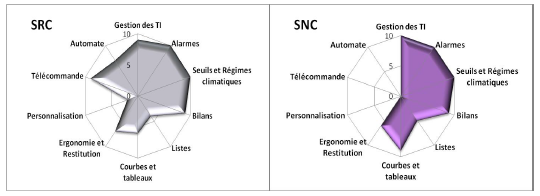
\includegraphics[width=0.7\textwidth]{0.figuras/Stanway_Kiviat_diagram_users.png}}
    \captionof{figure}{Kiviat diagram of STANWAY users. SRC and SNC are the highest level of automatons communications protocols at present.}
    \label{fig:Kiviat_StanWay_users}}
\end{figure}

\subsubsubsection{Apogee}
\label{sec:approach:project-approach:parties:apogee}

Tomorrow, driving systems must respond to an flexibilization and clients foreshight need. Apogeee seeks to redress this issue, and evolve the driving model towards a real-time managmenet navigation system, rather than an annual one. Apogee dispose several features for managing periodic maneuvers, parades, logging, reduction of losses or optimization of the network voltage plan, which will be subsequently taken over by Stanway.

\begin{figure}[h]
    \centering
    \parbox[t]{0.6\textwidth}{
    \href{http://collab.rte-france.com/SITES/cca/ref_architecture/AtRte/Pages/Accueil.aspx}{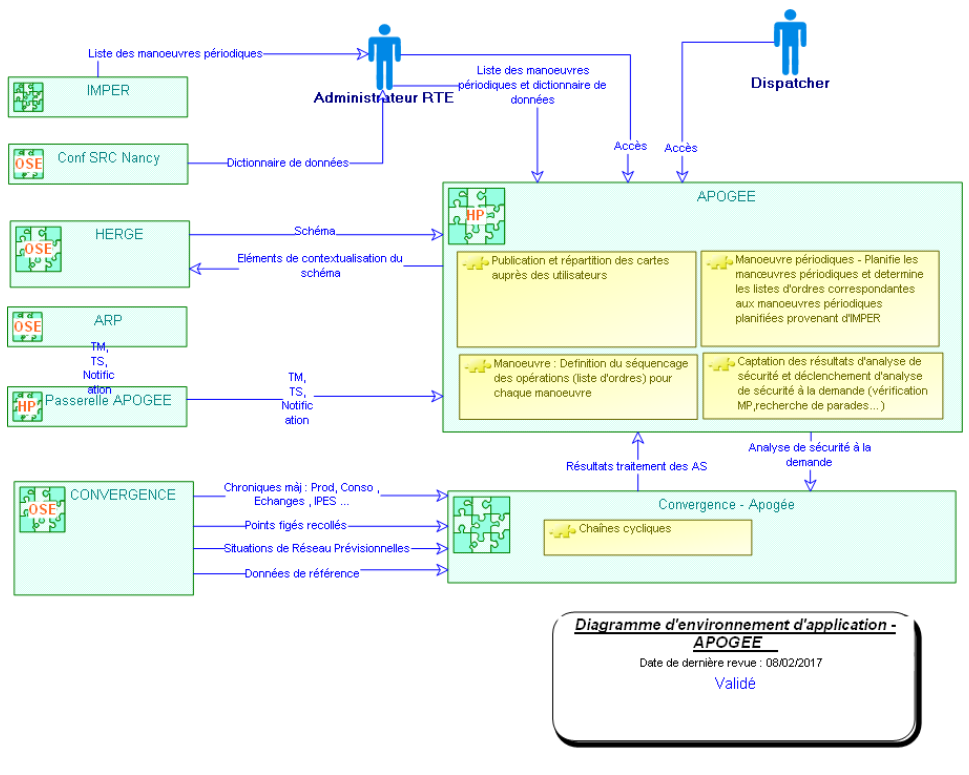
\includegraphics[width=0.6\textwidth]{0.figuras/diagram_APOGEE.png}}
    \captionof{figure}{Relational diagram between APOGEE \& HERGE. Click on the image to acces RTE's acronym database.}}
    \label{fig:APOGEE_diag}
\end{figure}

With a Java-software oriented approach\footnote{As most of the projects in the matter, Apogee was developed in Javascript. This providing feature performance advantages, their compatibility and flexibility remains notably inferior to FME's.}, Apogee opted for a much more user ergonomic canvass, where organs position may be modified to the user's taste after a primal page layout.

\begin{figure}[h]
    \centering
    \parbox[t]{0.45\textwidth}{
    \href{}{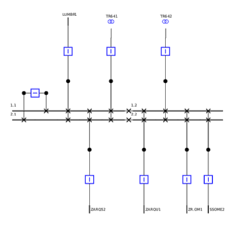
\includegraphics[width=0.45\textwidth]{0.figuras/TFM-Apogee-GAI.png}}
    \captionof{figure}{Prototype running in Apogee at Convergence.}}
    \label{fig:TFM-Apogee-GAI}
\end{figure}

\subsubsection{Risk assessement}
\label{subsub:introduction:thesis-purpose:risk-assessement}
On keeping with the aforementioned maxim, an additional difficulty pop up: notably, evaluating the impacts that the abovepresented concerned parties and others could have on the project's future. In this sense, several technical issues have been accordingly identified throughout the complete project, whom could be systematically approached and dealt with. Thus, a well-focused approach beforehand has decreased their impact and let to identify most of their consequences in advance.

Incertitude being well spread among different \nameref{subsub:introduction:thesis-purpose:project-approach:parties} on the modularity and adaptability have been the main maxima throughout the whole project, as result of a consequent risk assessment performed beforehand to the project.

As a result of this acknowledgement, \hyperref[fig:risk-matrix]{the following risk assessement matrix} charts the different inputs likely to impact the project, with an associated marginal weight on the project future scope: 

\begin{figure}[h!]
    \centering
    \parbox[t]{0.75\textwidth}{
    \href{}{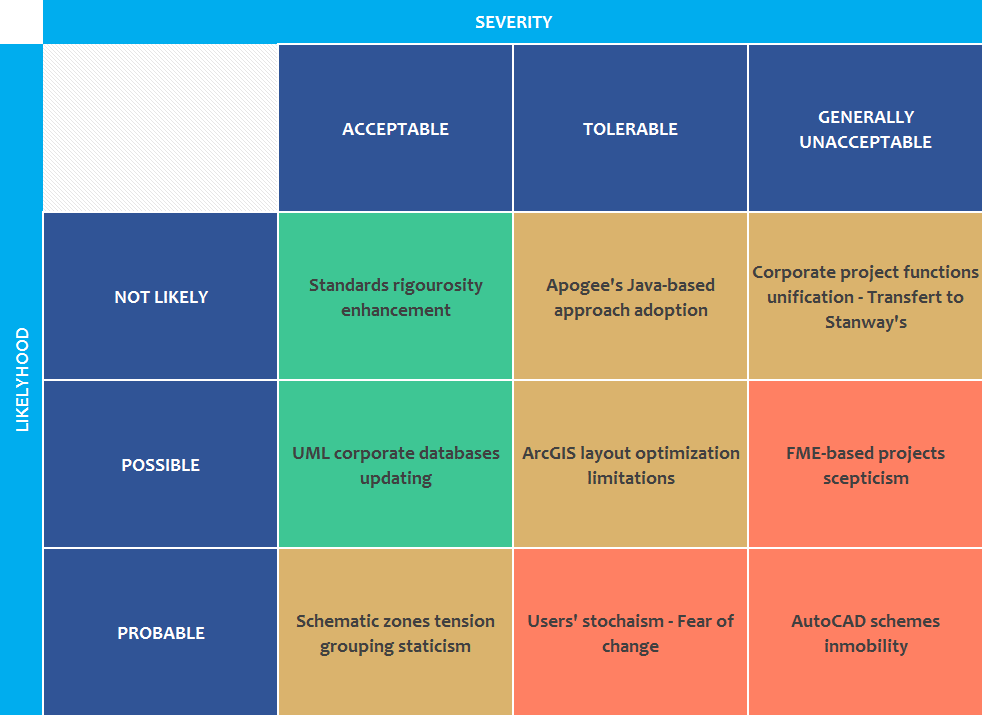
\includegraphics[width=0.75\textwidth]{0.figuras/risk-matrix.png}}
    \captionof{figure}{Hege risk matrix assessement.}
    \label{fig:risk-matrix}}
\end{figure}



% ---------------------------------------------------------------------

\subsection{Aim, scope and expected outcomes}
\label{sec:Intro:Thesis-purpose:Outcomes}
%REFORMULAR Y COMPLETAR

Digitalization is the order of the day in industrialization matters, although 15

On this pursuit, this project final aims to provide RTE with a comprehensible interface that could be extensible to multiple departments linked to SRC and SNC, and eventually enriched by the activities of STANWAY, APOGEE, ITESLA and other corporate projects embarked on the exploitation - real time management branch.
As sector trades are in continuous change in the last decade, tools digitization and data management is a constant in the matter and big companies as RTE must catch up the emerging technologies. Through all our contributions, we have intended to make the comings' work easier by providing them with a flexible and easily understandable network layout representation.  

Throughout all this document, it must remain clear to the reader what an important task lays on the rigorous and clear representation of the network. It will support most of the activities at ground level, where interdepartmental misunderstanding erupts as one of the major causes of fatal accidents in the sector. The latter delays the process development as all parts must be well concerned of any change and, therefore, corporate exemplars has to imperatively remain up to date. On top of that, numerous bureaucratic stages are internally stood so as to prevent for any error to take place \footnote{All them enriched simultaneously by the telecommute and telecontrol structure providing real time data of the network situation.}.

% ---------------------------------------------------------------------

% ---------------------------------------------------------------------


\chapter[Approach]{Approach}
\label{cap:Approach}
\begin{Resumen}

Within any industrial environment, a substantial and non-equivocate representation of the matter of study can be the most useful and time-saving tool, enabling performance boosting, yet as standardization. This chapter aims to illustrate the skill ramp-up performed so as to acquire and master the 2 main axes of the internship: i.e. \nameref{sec:approach:cim} and \nameref{sec:approach:software}, both required for convenient \nameref{sec:approach:project-approach} and contextualization.
\end{Resumen}
\PartialToc
\bigskip

\lettrine[lines=2]{\textbf{F}}{}rom the beginning of the \ingles{stage}, 2 principal axes were presented as main objectives of it, such as the \hyperref[sec:approach:cim]{Common Information Model (CIM)}, in addition to \hyperref[sec:approach:software]{all the sotware necessary} for its accomplishment: e.g. \nameref{sec:approach:software:matlab}, \nameref{sec:approach:software:FME} and the binomial  ESRI - \nameref{sec:approach:software:ArcGIS}.

\section{Introduction}
\label{sec:Diagram:intro}

These bidirectional objectives constituting a substantial skill rump-up, the first month and a half was basically framed on the familiarization with the tools and knowledge for such a purpose, and were aligning in the course of their learning. 

Indispensably, the author had to raise conscience of the problematic by gradually discretizing the problem and getting to get to know the departmental operation procedures, yet as the normative in the matter (specially regarding CIM schemes procedures). Once involved in the bureaucratic constraints implied, a theoretical introduction of the electrical devices seek to represent was stated.

Once the \ingles{Cahier des charges fonctionnel\footnote{Requirements specifications in french.}} stated, one was interested to the feasible technical solutions to sort it out. In the first instance, a \hyperref[sec:approach:software:matlab]{Matlab}-oriented approach was pursued, since the author felt much more comfortable with this tool. Those technical requirements going beyond the Matlab knowledge, project approach radically turned around, orienting towards the already used tools, and the departmental know-how, easing other members' skill transfer. 

Thereafter, the marked objectives visibility clarified notably, being two main axes the common thread of my project's contribution, from which certain structural sub-objectives could be identified:

\begin{itemize}
    \item \textbf{CIM}
    \begin{itemize}
        \item \textit{Familiarization:} 
        Becoming familiar with databases structuring and class arguments settlement is not easy and time-consuming.
        \item \textit{Standardization conscience-raise:}
        Standardizing any industrial application is a maximum if we want our project to remain accessible and functional in time and space.
        \item \textit{Normative constraints:} 
        Similarly, standardization objectives add difficulty to the problem, as they reduce its flexibility.
    \end{itemize}
    
    \item \textbf{Software deployment}
    \begin{itemize}
        \item\textit{Network model builder:} In charge oas seen inf databases-field assembling, by retaking class elements and re-affecting to those related in the fieldwork. Furthermore, hierarchical arboresecence confers the model its utility and veracity.
        \begin{itemize}
            \item FME: Powerfull Extract-Transform-Load (ETL) software for geographical, imagery and vectorial databases, used in data warehousing.
        \end{itemize}
        \item \textit{Displaying engine}
        \begin{itemize}
            \item ESRI: Being the world's most powerful mapping and analytics software, it furnishes with the best Geographic Information System (GIS) systems, such as ArcGIS or ArcMap. 
            \begin{itemize}
                \item \textit{ArcGIS} provides contextual tools for mapping and spatial reasoning and greater insights gaining by using contextual tools to visualize and analyze your data
            \end{itemize}
        \end{itemize}
    \end{itemize}
\end{itemize}

The sourcing quality of the virgin files used has deeply evolved along with the project. For that, an internal research was performed among the similar existing projects in Rte, successfully finding numerous adherence and certain exploitation possibilities. Thus, our original files, previously fed on completely chaotic and untidy RDF-formatted files, the exchanges with Stanway, then with Apogee have let us to base on much more relying and performant files. Whatsoever, files quality is still under study\footnote{An assessment study of Stanway's XML files' accuracy and rigurosity is currently being performed by ABB. Lille SRC's zone has already been validated, yet the rest of France remains under constant modifications.}, and  their evolution seems to be vital for the scrupulous representation of the entire France.

Once convinced of FME possibilities, a basic introduction to \nameref{sec:approach:cim} and \nameref{sec:approach:software:FME} conducted problematic awareness. Both FoS are quite technical and require lots of time for acquiring the technical competences at a professional level. The subsquent months supposed a continuous learning process and reciprocal contributions on more complexified matters (e.g. \nameref{sec:AIG:layout_optimization} techniques such as \nameref{subsub:AIG:SLV:graph_theory}, \nameref{subsub:AIG:SLV:MDS}, etc) from the individual to the project  and viceversa. These notions being implemented in \nameref{sec:approach:software:ArcGIS} toolset, and specially with \textit{Network Analyst}.

\begin{table}[h] \centering
\label{tab:margenes}
\caption{Month-to-month project time management procedure in weeks}
\begin{tabular}{lcc}
\toprule
\textbf{Project Time - Management template}  & & \\ \toprule
Phase description & Phase time(w) & Elapsed Time(w) \\ \midrule
Project dimension and finality acknowledgement & 1 & 1 \\
\textit{- First Matlab-driven post-level prototype} 	& 1.5 & 2.5\\
Reassessement & 1 & 3.5\\ \midrule
\textit{- Second Matlab-driven post-level prototype} & 1 & 4.5 \\
Software limitations awareness and reformulation &	2.5 & 7 \\ \midrule
FME skill ramp-up\footnote{This process has been markedly continuous and encompassed along the whole internship length.} &	2 & 9\\
\textit{- First FME Excel-driven zone-level prototype} & 1 & 10 \\
CIM corporate databases understanding &	1 & 11\\
\textit{- First FME CIM-driven zone-level prototype} & 2 & 13 \\ \midrule 
Standardization and Stanway know-how exchanges &	1 & 14 \\
\texttt{BusbarSection - Bay} notions - Modularization &	1 & 15\\
\textit{- Second FME CIM-driven zone-level prototype}& 0.5 & 15.5\\
\texttt{ACLineSegment} interposts notion introduction  & 0.25 & 15.75\\
Crossing-edges solution + ArcGIS interface dumping &	1.25 & 17\\ \midrule
\textit{- First ArcGIS zone-level prototype}&	0.5 & 17.5\\
Graph theory and layout management skills ramp-up & 1.5 & 19\\ 
FME position management import - looping &	1.75 & 20.75\\ \midrule
ArcGIS toolset (\textit{Network Analyst}) conscience raisement &	0.75 & 21.5\\ 
\textit{- First ArcGIS prototype} & 2.5 & 24\\ \midrule
Industrialization - Normative and reports writing & 2 & 26 \\
\midrule
\textbf{Total project time}& \textbf{26} &\textbf{26} \\
\bottomrule 
\end{tabular}
\end{table}

Time expended on each of these phases is specified in \href{the table hereafter}{tab:margenes}, for the reader to form a complete idea of how the pro jet evolved through project progress and personal skill ramp:

\begin{figure}[h]
    \centering
    \parbox[t]{1\textwidth}{
    \href{}{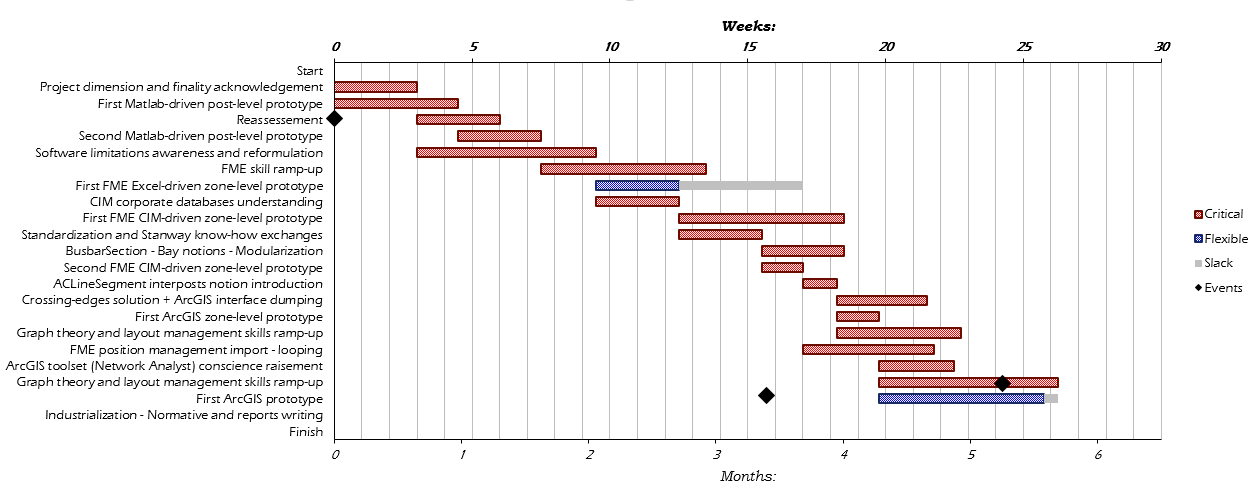
\includegraphics[width=1\textwidth]{0.figuras/Gantt-proejct.png}}
    \captionof{figure}{Gantt project management chart.}
    \label{fig:Gantt-diagram}}
\end{figure}

As in any project, its management seemed vital ff or resources optimizing and incertitude confronting. To this effect, a \hyperref[fig:Gantt-diagram]{Pert-Gantt chart binomial diagram} has been made in the incertitude phases of the project, assessing its control and tackling all the project long equally. To this effect, critical path and important tasks were identified constraining therefore their duration, yet as their potential impact in the whole project duration.

% ---------------------------------------------------------------------

\section{CIM}
\label{sec:approach:cim}

In electrical power industry, CIM refers to the standard developed by the International Electrotechnical Commission (IEC) and industrialized by Electric Power Research Institute (EPRI), with the support of the North American Electric Reliability Council (NERC), striving to normalize electrical network information exchanges between software applications\cite{IEC_CIM_static}. UML modeled IT environment, elements are represented as classes and any relationships between them are considered as associations. Inheritance allows specialization of common base elements into more specific derived elements.

From the perspective of Geographical Information Systems (GIS) users, CIM provides a useful data exchange schema for electrical objects \cite{CIMIntelliGrid}, and is of primary importance for layout support and communication with other applications. In addition, the paradigm shift around principal leading enterprises towards GIS network harvesting technologies enables CIM modeling harnessing for automatically reconstruct network diagram layout \cite{CIM-GIS}.

\subsection{Normative}

Through normalizing regulatory international framework, and in pursuit of databases standarization, application software integration is eased,  regarding any kind of energy transmission (explicited in \texttt{IEC 61970-301} \cite{IEC-2003}) and market communications (\texttt{IEC 62325}), normally portrait in  XML or RDF formats (\texttt{IEC 61970-501} \cite{IEC_xml-rdf} and \texttt{61970-452} \cite{IEC_CIM_static}).  

Ultimately, it is notably \texttt{IEC 61968} \cite{IEC-application} series of standards, plus the IEEE delivrables \cite{CIMIEE,CIMIntelliGrid} who extend CIM possibilities to meet the needs of electrical distribution in terms of distribution, work and outage management systems, planning, metering, geographic information system, asset management, customer information systems and enterprise resource planning. 

\subsection{Concept, utility and key aspects of CIM}

\textit{"An information model is a representation of concepts, relationships, constraints, rules, and operations to specify data semantics for a chosen domain of discourse"} (Y. Tina Lee, Information Modeling: From Design to Implementation, NIST, 1999): such an abstract definition enunciated 20 years ago remains completely valid on these days and perfectly depicts the proof of concept and interest of CIM, and of any Model Dreiven Architectures (MDA) logic generically. 

At that time, the need of a rigorous, logical yet versatile platform became increasingly apparent for massive data quantities management, notably on object regrouping and indexing, for better performance achievements, giving birth to multiple key dimensions that widespread in the recent years. Big Data, Intelligent behaviour or Internet of Things concepts are based on this concept.

Returning to the subject of CDL automatizing, by abstracting CIM knowledges, and applying them to the patrimonial databases, a double-sense impact on our study was obtanied: First it will contribute to the standarization of the patrimonial databases \cite{cahier_dpc2,guide_GAI,Note_accompagenement}, and secondly, it will decomplexifiy the problem, by clarifying the electrical elements to represent idiomatic structures. In our case, electrical elements were identified in different classes, as defined in \nameref{Acronyms} chapter. Each of them responding to a element on field and the most important being:

\begin{multicols}{3}
\begin{itemize}
\item \textit{ACLineSegment
\item BaseVoltage
\item Bay
\item Breaker
\item BusbarSection
\item ConnectivityNode
\item ConductingEquipement
\item Disconnector
\item EnergyConsumer
\item GeneratingUnit
\item Line 
\item LinearShuntCompensator
\item LoadBreakSwitch
\item PowerTransformer
\item PowerTransformerEnd
\item SynchronousMachine
\item Terminal
\item VoltageLevel}

\end{itemize}
\end{multicols}


Files initially used were RDF-structured, with linking chain attributes given in alphanumeric as those appearing in \hyperref[fig:RDFformat]{the following image}, where even though the introduction of a primer hierarchical notion was presented, one could nonetheless confer how absolutely no elements sorting and poor attributes enrichment was performed:


\begin{figure}[h]
    \centering
    \parbox[t]{0.6\textwidth}{
    \href{}{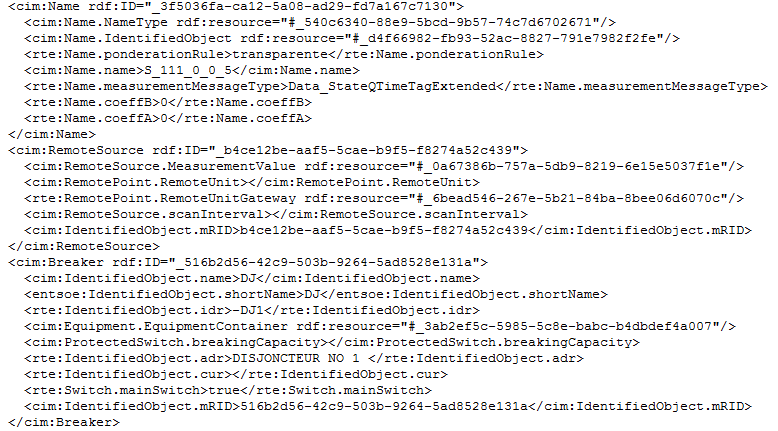
\includegraphics[width=0.6\textwidth]{0.figuras/RDF_database_format.png}}
    \captionof{figure}{Original RDF files appearance. A fragment from \texttt{GDP-AMIENS.rdf} displayed.}
    \label{fig:RDFformat}}
\end{figure}

This fact  notably contributing to data treatment engrossment and even often provoking data losses and rigorousness faibleness, a change to \hyperref[fig:XMLformat]{XML files} notably improved their clarity and structuring. Anyhow, the main hierarchical core of the treatment was maintained, whereas data quality fortly pare its complexity down. 

Thenafter, network elements were subsequently organized in different classes and characterized by their attributes in a ordered and logical way. Those classes being continent and content of others spawn an arborescent and structurally logical model, the metadata structure is transparent and bijective with regards to on-field architecture hierarchy.

\begin{figure}[h!]
    \centering
    \parbox[t]{0.8\textwidth}{
    \href{}{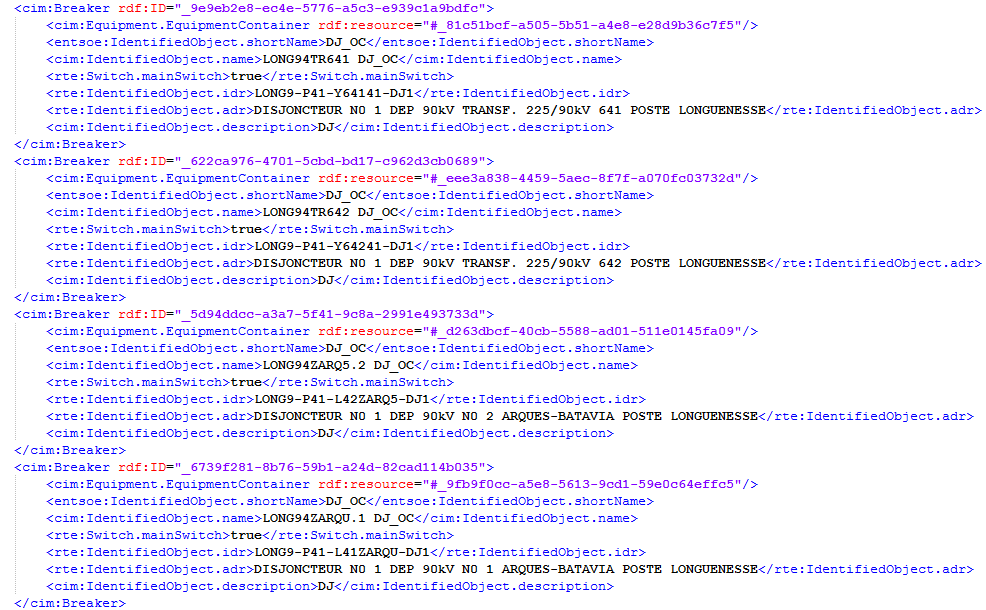
\includegraphics[width=0.8\textwidth]{0.figuras/XML_database_format.png}}
    \captionof{figure}{Stanway XML files appearance. Here, \textit{Breaker} class, from \texttt{V1-00-40-LILLE.xml} file is displayed.}
    \label{fig:XMLformat}}
\end{figure}

As it will be shown in deep all along \nameref{cap:AIG} chapter and particularly in \autoref{tab:classes_XML} is pretty well-illustrated, priorizing the classes as well as identifying relevant attributes to join all them is prior to understand and extend the UML model as it was conceived by the designer\cite{CIMIntelliGrid}. Those attributes (\textit{ACLine Segment, BusbarSection, Breaker, GeneratingUnit}) normally take unequivocally and hierarchically account of in-field switch-gear(which  will refer to an Intersubstatinons connection line, a Busbar, a Position breaker or a Power Generator reciprocally). Indeed, \autoref{fig:CIM_diagram-layout} enables to easily identify how the different topological structures contained in a 3-positions post, each of them pointing toward a different voltage level is non equivocally correlated to a different \textit{VoltageLevel}\footnote{Referring to the broken-line square regrouping the different tension levels (and not the \textit{PowerTransformer} nor the \textit{ACLineSegment} for example).}.

Attributes assembling and arranging, as deeply exploited in \nameref{subsubsec:AIG:methodology:structurisation:topology} sub-chapter, enabled discernive representation in \nameref{sec:approach:software:ArcGIS} through layers regrouping and intelligent displaying\footnote{Standards indicate than rates of 1000 objects-per-screen are adequate for a good discerning displaying.} optimization.

\subsection{Diagram layout}
\label{sec:approach:diagram_layout}

The ability to visualize network schematics can be critical for engineers when interpreting the status of an electrical network. As the number of interlocutors utilizing electrical models grows and utilities move towards a common network model across applications, the drive to ensure \hyperref[sec:approach:diagram_layout/SLD]{single line diagrams} are accurately reproduced in a standard and performant way sharpens progressively.

CDL format extends CIM to provide a mechanism for standardizing how the layout of electrical schematics is displayed, relaxing  graphics and network data exchange, while ensuring that schematic views are synchronized with the electrical model across multiple systems, such as \nameref{sec:approach:project-approach:parties:stanway}'s or \nameref{sec:approach:project-approach:parties:apogee}'s, regarding our corporate framework. In other words, this standard is intended to allow each of those system to accurately recreate the layout sought, by using their own styling for icons, colors, fonts and other graphical rendering attributes, while keeping their exceptional functionalities on the margins. 

\begin{figure}[h!]
    \centering
    \parbox[t]{0.7\textwidth}{
    \href{}{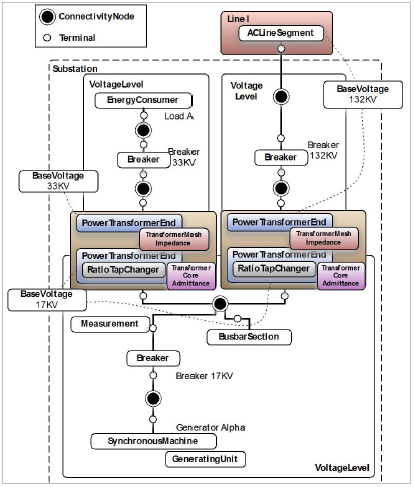
\includegraphics[width=0.7\textwidth]{0.figuras/example_CIM_mapping_UML-structure.png}}
    \captionof{figure}{CIM structural data skeleton and classes interdependances. Example Circuit with Partial CIM Class adjacences \cite{CIMIntelliGrid}.}
    \label{fig:CIM_diagram-layout-skeleton}}
\end{figure}

This way, elements can be systematically represented in common and standartized criterial specifications and, if sourced on the same patrimonial databases\footnote{as it is actually intending between Stanway's and Herge's at the momment.}, architectural structure of the represenation will be completely transposable, regardless of the particularities of each functional tool. To illustrate this fact, backtracking on the post representation subject, this structure could be extended and parametrised in such a way that the final representation of a certain post (retaken s seen in \autoref{fig:CIM_diagram-layout-skeleton} logic) will be the same and completely evident to the actual display, notably that of\hyperref[fig:CIM_diagram-layout]{the figure here below}.

On this pursuit, \textit{Terminal} and \textit{ConnectivityNode} notions are extremely important as they are in charge of the subsequent elements linking, specially when several attached to a similar post, as displayed in \autoref{fig:post_XML_structure-Terminal} in the following. Electrical network standards criteria has been respected in object representation, where different constraints have been established in pursuit of diagram layout adapting to the requirements specified in \cite{CIMIntelliGrid}.

\subsubsection{Single-line high voltage electric diagrams}
\label{sec:approach:diagram_layout:SLD}

Reducing the three-phase power system representation of the evoked example to SLD standards, the final appearance of the aggregated classes automatic and properly-ordered layout display would be as follows:

\begin{figure}[h!]
    \centering
    \parbox[t]{0.7\textwidth}{
    \href{}{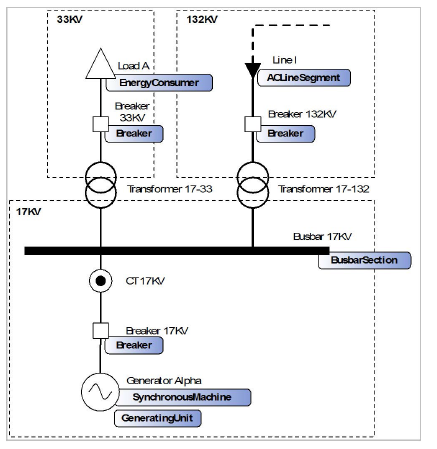
\includegraphics[width=0.7\textwidth]{0.figuras/example_CIM_mapping.png}}
    \captionof{figure}{CIM structure projection on diagram layout representation. Example Circuit with Partial CIM Class Mappings \cite{CIMIntelliGrid}.}
    \label{fig:CIM_diagram-layout}}
\end{figure}

Such a tedious task was traditionally performed by teams of architects who manually drew the complete SRC and SNC schematics in AutoCAD. In this, no optimization criteria was stated apart from the personal experience of the designer, which obviously, remained purely subjective. To this extent, several assessment criteria have been established in the wake of several meetings convened with \hyperref[sec:approach:project-approach:parties]{the different concerned parties} to identify common interests, as well as eventual divergences inter projects, and thus fix a common criteria consequentially. 

At any rate, all the stakeholders agreed that any automatizing could not be performed in a coherent extend unless international procedures regarding CIM database settlement and exploitation legislature \cite{CIMIntelliGrid, CIMIEE}, plus those existing on electrotechnical representation of HV schemes were totally respected individually and threaded together.

\subsubsection{Spread-out of technology impact on diagram representation}


is driving progress on this  integrated approach across
Several software applications have been traditionally used for functional design, physical design, and asset tracking, being \textit{Actrix Technical 2000}, from \textit{Autodesk}, and \textit{Visio 2000 Technical Edition}, from \textit{Microsoft} the most widely known. Nonetheless, few affordable software applications integrate all of these capabilities combining an interactive graphical interface with links to pertinent data for a comprehensive, yet easy-to-learn-and-use technical drawing environment.

That is the reason why numerous enterprises have been recently seduced by the idea of automatizing their corporate schemes through patrimonial databases plus Application Program Interface (API) tools exploitation. ORACLE,  JavaScript\cite{automatic-orthogonal-graph,CIMjava}, GIS programs... the demand on highly-skilled employees on the matter is definitely and remarkably growing, so does the identification of those needs. 

In addition, numerous technologies could benefit from the development of this, for the moment, merely-scientific-techniques on an industrialized approach, due to its transponability possibilities: \textit{Pajek} and \textit{Tulip} for big networks visualization \cite{aig-state-of-art-softwares} are the mainstream tools. Diagrams visualization can be performed static (\textit{Graphviz} (in multiple formats)) and dynamically (\textit{Dynagraph}), along with \textit{yFiles} for archives formatting, \textit{DBdraw} for Relational Databases or \textit{Govisual} for UML Class Diagrams, being most of this technologies developed in Eclipse Modelling Framework (EMF) platform.

Development of this software toolset is driving progress on this integrated approach across Business Process Model and Notation (BPMN) automatic layout \cite{automatic-layout-bpmn}, Assets adjustments on Mental Mapping \cite{layout-adjustement-mental-map}, automatic orthogonalistaion of graphs \cite{automatic-orthogonal-graph} or automatic similarity relationship assessment in bioinformatics \cite{algorithm-biological-data}.

ACERCAR LOS EJEMPLOS ALGO MAS A LO QUE HAGO YO => MEJORAR LA BUSQUEDA Y CAMBIAR LAS CITAS.

\section{Software deployment}
\label{sec:approach:software}

Acknowledging which tool meets our needs best comports a non-negligible marginal weight of the whole project success, yet it could even risk losing its route if a previous state-of-art effort is not undertaken. In my case, this stage took several time, as multiples possibilities in terms of software deployment seemed to be feasible, notwithstanding forget that my technical skills on the use of most of them chosen were more than poor at the beginning of the internship.

Thus, by shifting from an only Matlab interface prototype \nameref{sec:approach:software:matlab} to the final implementation of an intelligent, adaptable and performing representation system by using \nameref{sec:approach:software:FME} for the architectural part, and \nameref{sec:approach:software:ArcGIS} for the purpose of displaying optimization, the possibilities and perspectives of the project approached evolved considerably. Through all this software use, modularity has been a maximum prioritizing latters work restart and whole project industrialization.


Inter alia, those 2 software are mainly preponderant on the setting up of Herge's diagram layout automatizing, so are the stages in which this layout has been reached. In so doing, a first stage of data treatment and analyzing has been performed in \nameref{sec:approach:software:FME}, comprising this part the major part of the time passed. Secondly, a post-data treatment process resulting from \nameref{sec:approach:software:ArcGIS} activities took place, much less time consuming and evident, where post positions and even breakers' was modified so as to optimize the whole representation. Positions which were initially given by files extracted from DPC\textsuperscript{2}, and experimented several transformations thanks to the\nameref{subsub:AIG:SLV:graph_theory:meta_algorithms} implemented in \nameref{sec:approach:software:ArcGIS}. 

As recurrently cited, different files formatting were used all over the project, which was possible to the flexibilization of the entry-exit flux of data. This versatility was possible thanks to \hyperref[fig:FMEversatility]{FME's understanding capacity of the different formats imported}, and there sustains the  criteria decision of its choice. COMPLETAR

\subsection{Matlab}
\label{sec:approach:software:matlab}

In a first approach, the user felt much more confident on using Matlab for digital projection of the existing architecture on-field. Therefore was it chosen for a primal project requirements approach, enabling a conscience-raising in addition to a know-how corporate ramp-up. At any case, we must distinguish that the idea that Matlab was evidently not the proper software for the final implementation for the service was always acknowledged, although user was not yet technically aware enough for its correct implementation. 

The approach undertaken consisted on the creation of different post pictograph typologies through the use of several matrices disposition. This enforced technical knowledge on electrical devices semantics and their schematics while introducing the corporate post typologies gradually. Therefore post location and bar positions were reproduced, with a posterior patch that enabled their coupling.

\begin{figure}[h!]
    \bigskip
    \begin{center}
        \parbox[t]{.475\textwidth} {%
        \href{}
            {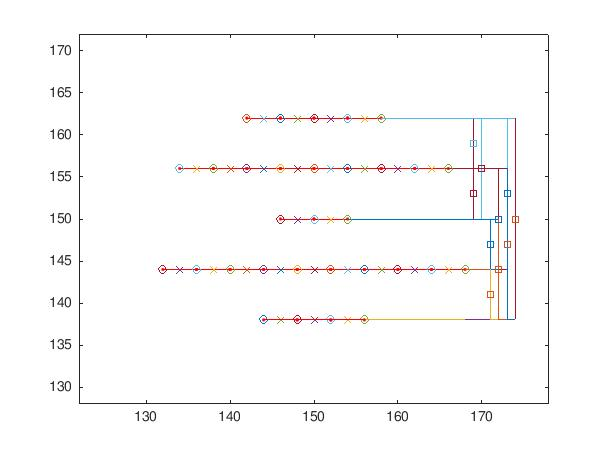
\includegraphics[width=.475\textwidth]{0.figuras/Matlab_postes_barres_generation.jpg}}}\hfill
        \parbox[t]{.475\textwidth}{\caption{Initial Matlab-oriented approach of a 5-barres-post design (all barres coupled).}
            \label{fig:matlab_design}}
    \end{center}
\end{figure}

Code is available on the \nameref{subsec:Appendix:Diagram:Matlab:code} subsection of Appendix. Its size and approach give full account of the limitations this canvass implied and so of the necessity of a more intelligent evolving perspective in term of software usage. 


\subsection{FME}
\label{sec:approach:software:FME}
That is, after a first Matlab-oriented approach (see \autoref{fig:matlab_design}), the author could thus raise conscience of the project dimension, and so that, of the necessity of a much more data-oriented software.

The major bulk of the work was performed using FME, began the moment the author introduced it on its data processing treatment, that is, at the beginning of the second month of the internship. With the worldwide mot used Spatial ETL application, the main part of the value-adding process aroused: thereafter, a new dimensional "thick-pipe"\footnote{Traditionally the software used to translate geographic data to a different format had limited capabilities. Most of the data would be forced through a limited data model causing much of the meaning to be lost in translation. We call this a “thin-pipe translation”.} translation method between databases integration on representation software became a reality.  

Spatial ETL tools can read, write, and manipulate spatial data (or not necessarily) in a whole array of supported semantic formats bijectively, streamlining data translation from one spatial database or GIS, CAD or raster graphics software to another. Those features were deeply exploited for posts representation in different coordinated systems inputting.

\begin{figure}[h!]
    \centering
    \parbox[t]{0.6\textwidth}{
    \href{https://www.safe.com/how-it-works/}{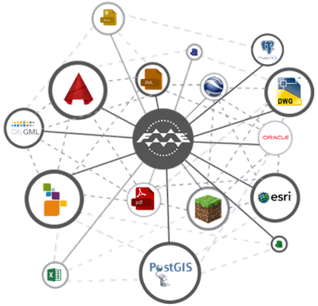
\includegraphics[width=0.6\textwidth]{0.figuras/FME_versatility.png}}
    \captionof{figure}{FME versatility leads to multiple format understanding possibilities}
    \label{fig:FMEversatility}}
\end{figure}

Plus, it offers a much more efficient and economic representation in terms of memory usage consumption, which, in view of the size of the files managed, implied a considerable computation power releasing of the processors corporative unit.
Furthermore, FME provides incredible performances in data consolidation and clarification, which strenghtened considerably blanks or incoherences presented on the imported XML files. Also, its online or and cloud working capabilities enabled multiples team working on a same file symustaniously and, what is more important, non concomitantly\footnote{In the futrure, \href{https://git-scm.com/}{Git}-formatted industrialization of the problem could enable multiple features introduction, such as versions controls or multiple users work enrichment.}. 

Outbound information form each treatment block is consecutively used and stocked in form of a blockchain\footnote{A block chain is a continuously growing list of records, called blocks, which are linked. Each block typically contains a cryptographic hash of the previous block, a timestamp, and transaction data.} tree, in which every block enriches the information contained in the chain. Those blocks being previously configurated and coded, make the class interusage activity much more intuitive. 

Given the high computational power needed, programs were run through a virtual machine (VM), whose IP, and therefore, whose server was shared among all the team members\footnote{Whatsoever, the team owned several VMs for different programs installation and launchment.}.

 
\subsection{ArcGIS}
\label{sec:approach:software:ArcGIS}

Currently, lots of controversy has been awaken since private geodata leaks are a never-end problem on the matter. Indeed, lots of software are capable of not only have access to our geographical position information, but also recross, parametrize or reassess it with others for assessing intelligent models of human behaviour, shortest-path opening business headquarters setting or automatic objects positioning for space optimization. \href{https://www.esri.com/en-us/arcgis/about-arcgis/overview}{ArcGIS, powered by ESRI} is the software used for pictographical projection of the previously FME-shaped network. By means of it, different infographies and images can be linked to FME objects class's typology, ensuring regulatory compliance. 
KEEP THE IMAGE??

\begin{figure}[h!]
    \centering
    \parbox[t]{0.8\textwidth}{
    \href{https://www.diatomenterprises.com/visual-data-representation-in-google-maps-bing-maps-or-esri-which-to-choose/}{
\includegraphics[width=0.8\textwidth]{0.figuras/googlemaps_bingmaps_esri.jpg}}
    \captionof{figure}{Representation systems are well spread among non-professional users. Google, Bing and other search engine have been including them on their mapping devices for some time now.}
    \label{fig:Googlemaps}}
\end{figure}

Geographical information coming from FME treatments was traditionally visualized with the integrated FME Data Inspector. Nevertheless, ArcGIS offers a much more efficient and economic representation in terms of memory usage consumption\footnote{In view of the size of the files managed, implied a considerable computation power releasing of the processors corporate unit}.

In addition, it enabled working with objects repositioning and their geographic information emerged, while improving displaying quality thanks to ArcReader performances. In particular, a vast range of enriched functionalities were systematically added to the process, chipping in the final result with some additional features. Thereby, several greater insights were gained by using contextual tools such as object layering thanks to ArcView and ArcEditor, which contributed to clarify the representation, while discretizing the object types, plus their adjacent information (ArcInfo) that was intended to be displayed, as well as it.

But what contributed the most to the problematic of study were ArcGIS spatial analytics features, which lead to spotting in the lattice network spatial patterns for more convenient redispositions, in the purpose of a certain objective funciton optimization. This algorithm, inspired in \nameref{subsub:AIG:SLV:graph_theory} principles, could be equally implemented in the future through on-field modifications with no-contribution  required (appart the patrimonial databases enrichement), as its setting up has been completely automatized.

ANADIR IMAGEN DE NETWORK ANALYST??

Real-time GIS empowers location monitoring for SCADA schemes, accelerating response times, optimizing safety, and improving operational awareness across all assets and activities, whether in motion or at rest. Moreover, data collection and management has been integrated in the corporate systems efficiently and securely.

Conversely, several issues were faced when geodatabase dumping between FME and ArcMap. This was due to the attributes formatting in the extracted document, which didn't always come from the same origin, so that their architecture and typology was neither. This ended up resulting on a non-canonical and unique data structuring. 

% ---------------------------------------------------------------------






\chapter[Automatic image generation] {Automatic image generation}
\label{cap:AIG}
\begin{Resumen}
AIG defines the ability to display any kind of graphical representation (e.g. images, pointers, schemes, etc.), based on data from any origin possible autonomously and faithfully.
\end{Resumen}
\PartialToc
\bigskip
\lettrine[lines=2]{\textbf{A}}{}utomatization of any element requires a complete and scrupulex knowledge of the original data, plus of the treatment undertaken with them. Therefore, its achievement has implied a long period of \nameref{sec:approach:software:FME} and \nameref{sec:approach:software:ArcGIS} traineeship, apart from a theoretical contents (\nameref{subsub:AIG:SLV:graph_theory}, \nameref{subsub:AIG:SLV:Voronoi} and \nameref{subsub:AIG:SLV:MDS} among others) projection towards its completion. Through a first vertebrance of the CIM file structure in FME, followed by a post-treatment image optimization performed in ArcGIS, the autor has ended up with an automatic, intelligent but still versatile and intelligent displaying process of the network layout entirely automatic. 

The openness towards performance optimizing processes altogether with the explosion of Big Data makes automatic image generation to be the order of the day in numerous engineering FoSs \cite{Software_diagrams, Deep_learning_image_to_text}. Notwithstanding, when we extrapolate this to the corporate network layout of the big electrics most of this reports are strictly confidential and merely code-oriented \cite{standard-based-SLD-AG,}. This fact forces to a severe abstraction exercise to take place, seeking to adapt the state of art actual innovations to our case of study. 

At the moment, we are deeply surrounded by intelligent AIG devices, able to mutate in function of a certain parametrization: DAR EJEMPLOS DE AIG. This unperennity recognition process is called as \nameref{subsub:AIG:SLV:graph_theory:meta_algorithms}, a variable evolution of \nameref{sub:AIG:machine_learning} ethics, giving borth to the term Automatic Machine Learning (AML). 

At the moment, multiple softwares (\hyperlink{https://github.com/iTransformers/netTransformer}{netTransformer}, \hyperlink{https://github.com/OpenNMS/opennms}{OpenNMS}, \hyperlink{https://www.docusnap.com}{Docusnap}\footnote{This licence-restricted software is also XML-based, so is our methodology.} or \hyperlink{https://www.netbraintech.com}{netBrain} among others) have been developed to easy the representation of all topologies of network diagrams. However, they remain power-limited and with a low level of automatization in regards to the requirements of Herge.


\section{Introduction}

Automatic electrical network layout generation is introduced in this work. In general, the proposed \nameref{sec:AIG:methodology} has potential in functional software testing and industrialization. The present study was pursued on the basis of the actual widget, with an aim on its automatizing, but still making use of the same corporate methods, software and principles.

Several steps were taken to progressively attack the challenge in the most rigorous manner:
\begin{description}
    
    \item - A \textbf{skill ramp-up} let the author technically identify the different elements of the electrical network in the field, and the way they were represented following corporate conventions \cite{doctrine_cod_sites, doctrine_cod_liaisons, doctrine_cod_postes}.
    
    \item - Thereupon, \textbf{taking conscience of \nameref{sec:approach:software:FME} potential}, while impregnating of its working methodology was the roughest step. Different case studies were performed to project mental skills on problem solving through this software, which progressively increased in difficulty.
    
    \item - Once FME-capable of exploiting the problem, a \textbf{familiarization with the databases}, their alphanumeric argument coding system and the way they were structured was carried out. This databases were enriched subsequently for easing meetings' agreements to achieve the bijectivity between them and the different elements representation.
    
    \item - The network skeleton once completely displayed, \textbf{image optimization processes} could begin. Different theoretical solutions were envisaged \cite{Genetic_algorithms, AlgoAIG}, to serve as a basis for \nameref{cap:AIG:diagram:ArcGIS}'s subsequent use in image performance optimization by objects reordering. 

\end{description}

Finally, an adequate \textbf{transfert of knowledge} is in course for the project life to extend. For this reason, several corporate guides have been written illustrating the approach undertaken.

\section{Objective}

In the wake of completely automatize Herge's scheme displaying, several objectives had been set by the author at the beginning of the traineeship, in form of a sort of specifications requirement document. Not static and strictly linked to the tools availability, those specifications are as follows:

\begin{enumerate}
	
	\item First of all, the final but of the work was to \textbf{provide Herge with a changing interface}, able enough to adapt itself to the coming changes in the next 5 to 10 years.
	
	\item Secondly, the \textbf{requirements fulfillment had to remain untouched at any change} introduced. That is, the bargaining power of the clients constantly marked the guiding thread of the project. Several meetings were animated with the person in charge to reframe projet's scope and budgeting.
	
	\item Thirdly, \textbf{interactions among projects} had to be taken into account. Projects' leeways represent one of the main causes of money and time waste in the actual enterprises world. 
	
	\item Fourth, the technical process skeleton remains \textbf{the most versatile for the changing sourcing or goals light differs} to remain technically feasible. Several software have been used throughout the project to draw nearer to every step requirements of the project.
	
	\item And lastly, all the \textbf{work} undertaken must be \textbf{properly documented} for the comings to easily comprehend its establishment and retake it profitably. Pursuing so, the decisions taken and the progress-making approach sticks to the basics in to an intuitive way.
	
\end{enumerate}

Summarizing, the objective is to provide Rte with a rigorous, still technically feasible solution: that is, an adaptable network diagram layout automatic generator by using their corporate databases and their software tools in an intuitive way to be easily retaken in the future, still while strictly satisfying clients requirements.


\section{Normative}
\label{sub:AIG:normative}

A vast range of literature can be found on any electrical regulatory framework FoS, due to the high level of industrialization in the matter and the incredible development the sector has been experiencing in the last decades. However, principles vary considerably from one another, as it is finally the enterprise know-how which inspires the global approach of their drafting.

In parallel, and throughout all this process, several corporate livrables have been of great use in AIG implementation, driven by the Rte mainstream voices \cite{guide_GAI,Infos_GAI,specif_detaillees_GAI} and by several contacted delivers, such as Thales \cite{gai_thales}.

\subsubsection{CIM regulatory framework}
\label{subsub:AIG:noramtive:CIM-framework}
\texttt{IEC 61970} has encompassed the mainstream line for this internship, guiding and establishing on technical matters all the necessary conventions for proper industrialization of the approach, as the training agreement specified in a first term.
For proper discretization among literature, a extremely useful guideline is Common Grid Model Exchange Standard (CGMES)   \href{https://docstore.entsoe.eu/Documents/CIM_documents/Grid_Model_CIM/140528_ENTSOE_CGMES_v2.4.14.pdf}{hereafter}:

\begin{itemize}
\begin{itemize}
\item  \textbf{\ttfamily {IEC-TR 61970}: Standard.}These series of standards deals with the application program interfaces (APIs) for energy management systems (EMSs).
\begin{itemize}
\item \textit{IEC 61970-552:} CIM XML Model Exchange Format
\item \textit{IEC 61970-301:} Common Information Model (CIM) Base
\item \textit{IEC 61970-302:} Common Information Model (CIM) for Dynamics Specification
\item \textit{IEC 61970-452:} CIM Static Transmission Network Model Profiles
\item \textit{IEC 61970-453:} Diagram Layout Profile
\item \textit{IEC 61970-456:} Solved Power System State Profiles
\item \textit{IEC 61970-457:} Common Information Model (CIM) for Dynamics Profile
\end{itemize}
\item \textbf{\ttfamily{IEC 61968-4}}: Application integration at electric utilities – System interfaces for distribution management - Part 4: Interfaces for records and asset management.
\item  \textbf{\ttfamily {DSP0004}}: Common Information Model (CIM) Infrastructure
\end{itemize}
\end{itemize}

\subsubsection{Electrical devices representation}
\label{subsub:AIG:normative:elec-representation}

Among the regulatory documentation spectrum regarding electrical objects symbolic representation, 3 superposing plans (\textit{International, french national} and \textit{Other regulatory documents}) may be differentiated in terms of competences and applicability derived from its requirements. 

\begin{itemize}
    \item \textbf{International regulation}
    \begin{itemize}
    \item \textbf{\ttfamily{IEEE Std 315-1975: Standard.} (Reaffirmed 1993):} Graphic Symbols for Electrical and Electronics Diagrams (Including Reference Designation Letters)
\item \textbf{\ttfamily {IEC-TR 62357}: Standard.}
        Major law in HV electrical diagram drawing. 
\item \textbf{\ttfamily{IEC 60617}:} Graphic Symbols for Electrical Diagrams 
\item \textbf{\ttfamily{IEC 61082}:} Electrotechnic documents and schemes establishment.
\item\textbf{\ttfamily{ISO 81714-1}:} 
Design of graphical symbols for use in the technical documentation of products
\item\textbf{\ttfamily{ANSI Y32.2.}:} 
Graphic Symbols for Electrical and Electronics Diagrams
\item \textbf{\ttfamily{ENA ER P-2/6}:} Engineering recommendation. Electricity distribution network planning design.


    \end{itemize}

    \item{\textbf{French national regulation}}
    \begin{itemize} 
\item \textbf{\ttfamily{NF EN 60617-2 (1996)} – Partie 2 :} Éléments de symboles,
symboles distinctifs et autres symboles d’application générale.
\item \textbf{\ttfamily{NF EN 60617-11 (1996)} – Partie 11 :} Schémas et plans
d’installation architecturaux et topographiques.
\item \textbf{\ttfamily{NF EN 81714-2 (1998)}:} Computer and library coding symbols and transmission.
\item \textbf{\ttfamily{FR1100}:} Technical Drawing (all parts)
\item \textbf{\ttfamily{FR1102.101}:} Electrical Symbols
    
 \end{itemize}
\item{\textbf{Other regulatory documents}}
\begin{itemize} 
       
 \item \textbf{\ttfamily{R357929}:} Drawing Management (Australian standard)
 \item\textbf{\ttfamily{R280697}:} General Substation Requirements (Australian standard)
\item\textbf{\ttfamily{R358449}:} Site Names and Abbreviations (Australian standard)
\item \textbf{\ttfamily{R280718}:} Transmission Line and Cable Numbers (Australian standard)
\item \textbf{\ttfamily{R280717}:} Transmission Circuit Name Abbreviations (Australian standard)
\item \textbf{\ttfamily{R280703}:} Asset Identification (Australian standard)
\item \textbf{\ttfamily{R280754}:} Site Drawing Prefix Master List
\item \textbf{\ttfamily{R358302}:} Drawing Checking and Approval Authorisation Guidelines
\item \textbf{\ttfamily{TSD-SD-806-0001-001}:} Drawing Symbols Drawing

    \end{itemize}
\end{itemize}

\subsubsection{Layout optimization regulatory framework}


Nevertheless, appart \texttt{IEC 61970-453: Diagram Layout Profile} standard, the regulatory framework is relatively inaccurate when referring to \nameref{sec:approach:diagram_layout:SLD} automatic optimization procedures. In this sense, theoretical principles remain unframed in an industrialized sense, which implies that no standards are found for \nameref{subsub:AIG:SLV:graph_theory} application in the context of study. Paradoxically, this procedures have been extensively explored and documented by researching centers evoking most suitable path, network engrossing office or flux transfer optimization problematic resolutions in the literature. INSERTAR CITAS DE LA TEORIA DE GRAFOS \cite{}.


\section{Proof of concept}

This section, constituting one of the most important of the chapter, yet of the whole thesis, aims to outline more precisely the client adaptive process. The subsequential Proof of Concept (PoC) process undergone, animated by a first required improvements identification, plus a technical methodology assessment process, whose main milestones can be found hereafter:

In principle, the department seeked to automatize, anticipation future requirements, the representation of the schemes used by on-field operators for a more logical and profitable gait to understand the network topology during operations to proceed for the daily practice of their professions. Out of this statement, two main objectives were declined directly: 
\begin{itemize}
    \item At first, clarity and \textbf{logical surveillance regarding the ancient schemes} was vital for the future support transverse of exploitation workers. consequently, ancient post positioning system was respected at maximum, as well as iconic and pictographic conventions.
    \item Secondly, for the purpose of \textbf{Herge scheme displaying automatizing} meaning database sourcing for architecture reproduction, a common model choice, plus its industrial exploitation had to be stipulated. In the light of this purpose, CIM database corporate models were seeked and exploited, so that elements representation was exhaustive as logical. 
\end{itemize}

Projecting these targets on \textbf{technical requirements terms}, a considerable evolution has been performed in terms of scope and software capacities: In so doing, after a first Matlab-oriented approach (see figure \ref{fig:matlab_design}), the author could thus raise conscience of the project dimension, and so that, of the necessity of a much more data-oriented software. 
Following several discussions for keeping the project scope on track, a radical technical approach changeover was undertaken: that is, a completely Matlab-sourced prototype was not due to encompass industrialization steps in the representation of a exhaustive and non-perennial corporate network layout.

This finally resulting in FME introduction, which would be explained in detail in section \ref{sec:approach:software:FME}, and without whom this project could have no longer ended up successfully. Completed functionality being possibly achieved in a 6-to-9 month range, thanks to the \textbf{accuracy and rigorousness of the databases sourcing}\footnote{Which had been completely update following normalization requirements \cite{CIMIEE}}, provided by StanWay following several meetings, that is what gives sense to the FME use. On top of that, a software already implemented and well-installed in the department know-how, at the expense of other different options, such as Java or Matlab coding, considered in a first approach.

Even so, users approval is necessary for the project practical transposition, although input - Stanway CIM files - and output - HERGE's corporative schema in DWL - interfaces are easily feasible, thanks to \textbf{FME versatility}, which will all at once remain as the main architectural CIM model reframer into a coherent diagram layout representation. In addition, its displaying could be optimized by the implementation of \nameref{sub:AIG:SLV:theoretical background} basis on \textbf{\nameref{sec:approach:software:ArcGIS}}, whose workbench tools (and notably \textit{Network Analyst} package) have been already successfully proved through similar projects.

\section{Methodology}
\label{sec:AIG:methodology}

Several stages have canalized the unifying idea of the project as the author improved his skills, which made project PoC feasibility notably evolve, and finally so did its expectancies too. Matlab, Java, FME, ArcGIS, etc.: lots of alternatives and softwares have been exploited and crossed altogether with a continuous scope reframing for squeezing all available means out and approaching the technical solution to the clients prospects the most, and more importantly, in a perennial way from now on.

In a first term, a didactic procedural introduction \nameref{sec:intro:AIG:structurisation} of the different \nameref{sec:intro:AIG:structurisation:classes} is performed, just as their \nameref{sec:intro:AIG:structurisation:functional-dependencies}, followed by a \nameref{subsubsec:AIG:methodology:structurisation:topology} of the different on-field elements typologies are tackled below.

The second subsection deals specifically with the \nameref{sub:AIG:data-management}, through a versatile range of \nameref{subsub:AIG:data-management:FME-fonct}.

Methodological explanation has been intended to be as didactic as possible, while staying technical enough for reporting on the edge-cutting contributions proposed and enriching any profile of reader possible. This two main stages will be systematically approached and developed so that the reader can follow the rational processes involved under the databases management, yet at the layout representation.

\subsection{Data structuring}
\label{sec:intro:AIG:structurisation}

As CIM regulatory standards \cite{IEC_CIM_static, IEC_CIM_convention} require, arguments structuring must be performed in a modular and interconnected way. Notably regarding electrical network elements sourcing \cite{IEC_xml-rdf}, the data classes must be declared as they are on field, thus keeping arborescent notion throughout the whole logic.

All this processus having been interiorized, then massively performed in FME, it is there where the major applicability possibilities to Herge in the short term relay, as it could eventually allow to automatically retake the network structure without necessarily affecting on the network layout display, and therefore without awaking users' complaints.

\subsubsection{Object classes identification}
\label{sec:intro:AIG:structurisation:classes}

A non-equivocal bijective relation is sustained between switchgear at ground level and classes in the UML model\footnote{except for low-architecture logic making levels (e.g. those of \textit{Terminal} or \textit{ConnectivityNode} in particular), where no physical notion exists}. In addition, each class comport several arguments that permit to identify and enrich representation characteristics in a modularized way, as \ref{tab:classes_XML} perfectly illustrates, leading sometimes to the characterization of its pictographical layout representation into a post-introspective perspective.

Towards data modeling constructions, several steps subsuming the bulk of the work undertaken can be easily differentiated. Everyone of them apporting a new feature and logically linked to the previous, they are systematically approached hereunder: 

\begin{itemize}

\item Identification of the different elements topologies and characteristics of the databases modeling classes, which are as follows:
\end{itemize}


\begin{table}[h]    \centering
\label{tab:classes_XML}
\caption{XML classes and their depending attributes}
\begin{tabular}{l|l}
\toprule
\textbf{Class} & \textbf{Attribute} \\ \midrule
ACLineSegment & ID \\
Bay & ID - bayOrderNumber - orientation - VoltageLevel \\
Breaker & ID - EquipementContainer \\
BusbarSection & ID - EquipementContainer - graphicPosition\\
Disconnector & ID - EquipementContainer \\
Line & ID \\
LinearShuntCompensator & ID - EquipementContainer \\
PowerTransformer & ID \\
PowerTransformerEnd & ID - PowerTransformer - BaseVoltage - Terminal \\
Substation & ID - Region \\
Terminal & ID - EquipementContainer - ConnectivityNode \\
VoltageLevel & ID - BaseVoltage - SubStation\\ 
\bottomrule
\end{tabular}
\end{table}

\subsubsection{Functional dependencies}
\label{sec:intro:AIG:structurisation:functional-dependencies}

Once the main attributes identified, we proceeded to establish linking bounds between main classes, to create the database UML model\footnote{Which will be possibly operable by \textit{Enterprise Architect} for corporate use.} cobweb.

Hereafter, the reader will find a synoptical diagram of the bounding links presented among them. Those dependencies will be set up thanks to internal tool packages, thoseprocedures been explited in deep in  \nameref{subsub:AIG:data-management:FME-fonct} section. In addition, attributes between different classes are not normally called the same way, and indeed it is the containing of the higher-leveled one that contains the key identifier of the one contained in the first mentioned, in alphanumeric format. This way, provided class identifier is unique will guarantee unity spread throughout the whole scheme.

\begin{figure}[h]
    \centering
    \parbox[t]{1\textwidth}{
    {\centering
    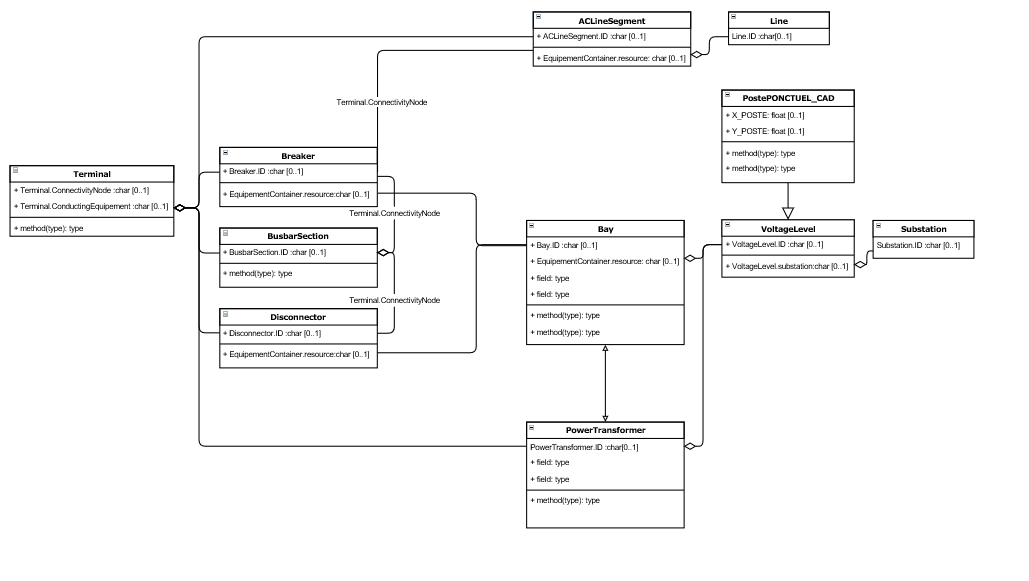
\includegraphics[width=1\textwidth]{0.figuras/Synoptique_UML_classes_RDF_Stanway.png}}
    \captionof{figure}{Classes synoptical dependencies diagram.}
    \label{fig:Classes-synoptical}}
\end{figure}  

On the pursuit of treatment power economizing, just those attributes specifically used for topological structure reconstruction are kept. On top of that, those associated with pictographical properties are evidently kept as well.

Even the lmogic structturing was pretty well formatted and discretional, no support of its UML model was in us. Henceforwarth, its deployment and reconstruction of the Stanway-imported files has been handmade reproduced by cognitive appreciation. 

\subsubsection{Topology reconstruction}
\label{}

Each of these elements classes corresponding to an electric notion (\textit{Breakers, Disconnector, PowerTransformer,} etc.), they are subsequently levelled, then regrouped  and, finally, enriched, as on-field. These dependencies an architecture deployment enabling to parametrize their representation, as shown in \autoref{fig:post_draft}.

\label{subsubsec:AIG:methodology:structurisation:topology}
\begin{itemize}
    \item Henceforth, classes are firstly hierarchically organized in several levels, as in practice, following the criteria shown in the \autoref{tab:classes_XML} below. These levels notion is quite important as it approaches the architecture skeletom to reality's.
\end{itemize}


\begin{table}[h]        \centering
\label{tab:classes_dependences}
\caption{XML classes hierarchical levels and depending attributs}
\begin{tabular}{l|l|l}
\textbf{\textit{Level}} & \textbf{Container} & \textbf{Contained}\\ \midrule
\textit{Lv.4} & Region & SubStation \\ \midrule
\textit{Lv.3} & SubStation & VoltageLevel \\ \midrule
& PowerTransformer & PowerTransformerEnd - Terminal \\
\textit{Lv.2} & ACLineSegment & Line - Terminal \\ 
& VoltageLevel & Bay - BusBarsection \\ \midrule
\textit{Lv.1} & Bay & Disconnector - Breaker - LinearShuntCompensator\\ \midrule
\textit{Lv.0} & Terminal & EquipementContanier - ConnectivityNode\\
\bottomrule
\end{tabular}
\end{table}

\begin{itemize}[label={}]
    \item The hierarchic model present in the XML databases model is built in such a way that every element is kept in relation with those form which it depends along the hierarchic chain, enabling attribute interlying and correspondence easy identification.
\end{itemize}


\begin{itemize}
  \item  Next, once the elements in \autoref{tab:classes_XML} identified, we proceed to the study of their functional dependence and continence relations in connection through \hyperref[fig:post_XML_structure-Terminal]{a coming good representation basis settlement}:
  \end{itemize}
\begin{figure}[h]
    \centering
    \parbox[t]{0.6\textwidth}{
    {\centering
    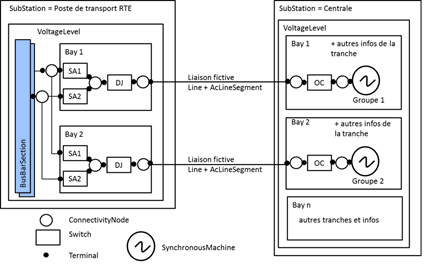
\includegraphics[width=0.6\textwidth]{0.figuras/BusbarSection_dependences_fonctionelles.png}}
    \captionof{figure}{Functional dependencies inside a post, according to XML-hierarchical tree structuring.}
    \label{fig:post_XML_structure}}
\end{figure}



  
    
    \begin{itemize}
        \begin{itemize}
            \item Here is where the \texttt{Terminal} notion appears, extremely important for keeping model connectivity.
       \end{itemize}
    \end{itemize}

\begin{figure}[h]
    \centering
    \parbox[t]{0.6\textwidth}{
    {\centering
    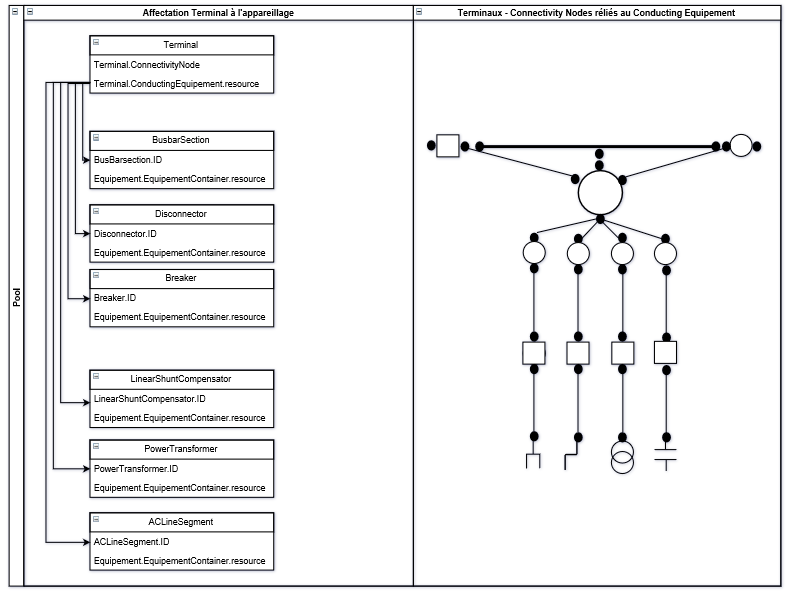
\includegraphics[width=0.6\textwidth]{0.figuras/Connectivite_classes-Notion_Terminal.png}}
    \captionof{figure}{Functional dependencies inside a post, according to XML-hierarchical tree structuring.}
    \label{fig:post_XML_structure-Terminal}}
\end{figure}  

\begin{itemize}[label={}]
        \begin{itemize}[label={}]
\item  As shown in the \autoref{fig:post_XML_structure-Terminal}, elements are not linked directly between them. A terminal let
bus multiple elements interconnection, and, by the way, its introduction clarifies intra-bay dependencies by adding an intermediate stage.
 \end{itemize}
    \end{itemize}
\begin{itemize}[label={}]
        \begin{itemize}
\item \textit{ConnectivityNode} as linker, and \textit{EquipementContainer} as continent let the forming objects to establish 2-way dependencies, as shown in \autoref{fig:Terminal-ConnectivityNode} for the third \textit{BusbarSection} of \texttt{SV.O-P71}, \textit{Saint-Valentin} 400-kV post third bar's (see \autoref{fig:post_draft}).
        \end{itemize}
    \end{itemize}

    \begin{figure}[h]
    \centering
    \parbox[t]{0.6\textwidth}{
    {\centering
    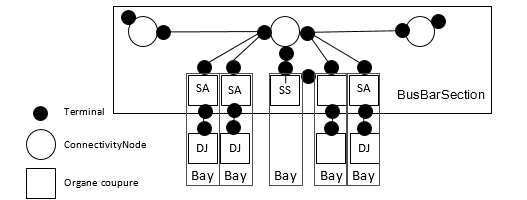
\includegraphics[width=0.6\textwidth]{0.figuras/Terminal_connectivityNode.png}}
    \captionof{figure}{\textit{Terminal} and \textit{ConnectivityNode} notions.}
    \label{fig:Terminal-ConnectivityNode}}
\end{figure}

\begin{itemize}[label={}]
        \begin{itemize}
\item On the basis that a\textit{Bays} and \textit{BusbarSections} are the standard continents of electrical switching devices, thus of \textit{Breakers} and \textit{Disconnectors} in the majority of cases, finally linked between them through \textit{Terminals}. 

\textit{Bays} are destined to represent positions towards other post, and thus their topological structure remains practically unchangable from the \textit{Disconnector-Bay-Disconnector} towards the object off-\textit{VoltageLevel}, whereas \textit{BusBarSections} can be unconcernedly linked by \textit{Breakers} or \textit{Disconnectors}, which will be affected to both terminals of the linking barres in question.

Finally, the topology inter-\textit{BusbarSections} is quite particular, where no notion of continance between the bar switchers and the bar themselves is explicted. 

\end{itemize}


\end{itemize}

  \begin{figure}[ht]
    \centering
    \parbox[t]{0.475\textwidth}{
    {\centering
    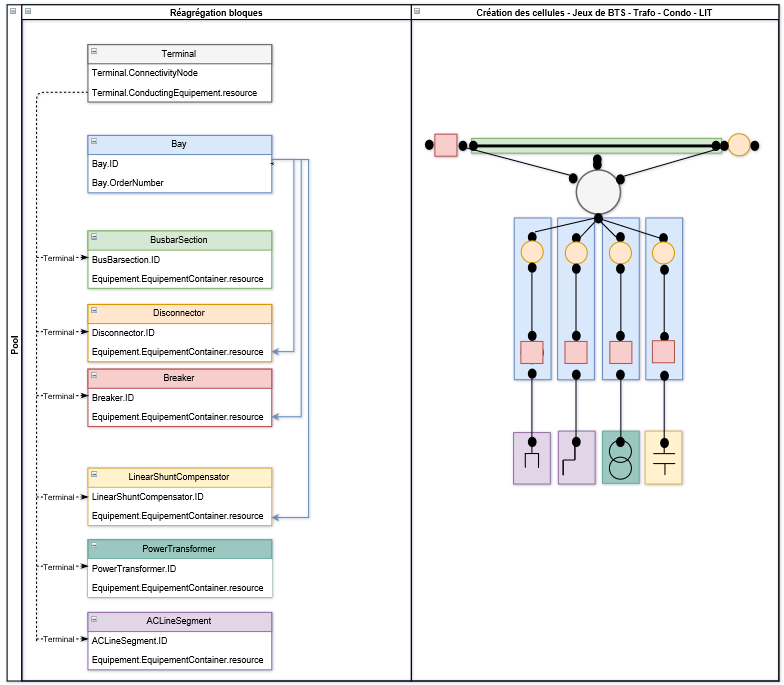
\includegraphics[width=0.475\textwidth]{0.figuras/Cellule_BTS_accroches.png}}
    \captionof{figure}{\textit{Bay} and its containing, plus \textit{BusbarSection} notions.}
    \label{fig:Bay_BusbarSection}
    }
    \hfill
    \parbox[t]{0.475\textwidth}{
    {\centering
    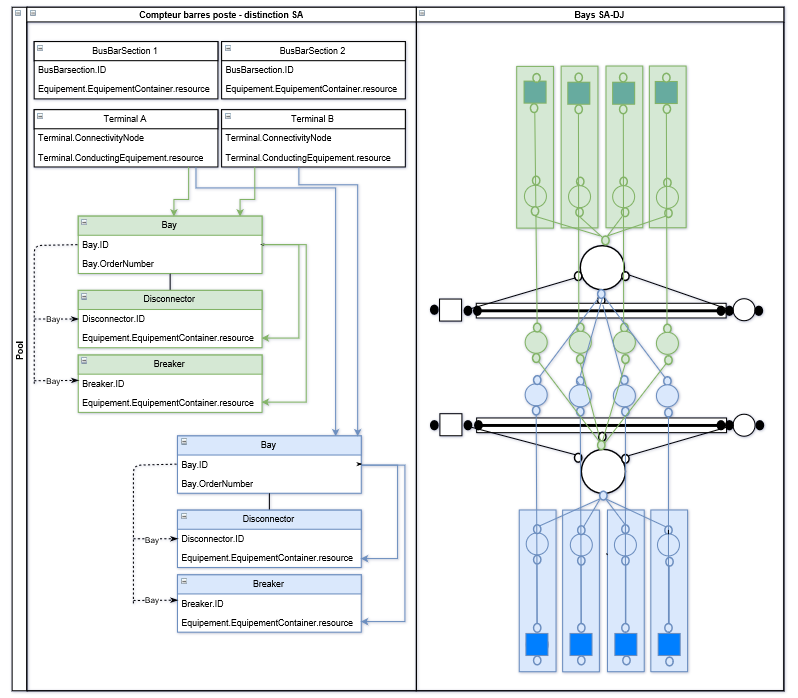
\includegraphics[width=0.475\textwidth]{0.figuras/Union_DJ-SA-Barre.png}}
    \captionof{figure}{\textit{Breakers} are affected to each \textit{Bay - BusbarSection} through \textit{Disconnectors}.}
    \label{fig:Breakers}
    }
\end{figure}

\begin{itemize}[label={}]
        \begin{itemize}
\item To illustrate this example onto group dependencies creation, the same way \textit{Bays} regroup \textit{Disconnector} and \textit{Breakers}, a post (\textit{VoltageLevel}) will contain the abovementioned \textit{Bay} notion, plus \textit{BusBarsection} one. 
\end{itemize}
\end{itemize}


\begin{itemize}[label={}]
        \begin{itemize}[label={}]
 Different \textit{VoltageLevels} are linked, as on field, by \textit{ACLineSegments or PowerTransformers}. Those last been a bit more complex, they include two "terminals" at each of their ends, which are contained in the \textit{VoltageLevel} and are grouped down the class of \textit{PowerTransformerEnd}. 
\end{itemize}
\end{itemize}

\begin{figure}[h]
    \centering
    \parbox[t]{0.475\textwidth}{
    {\centering
    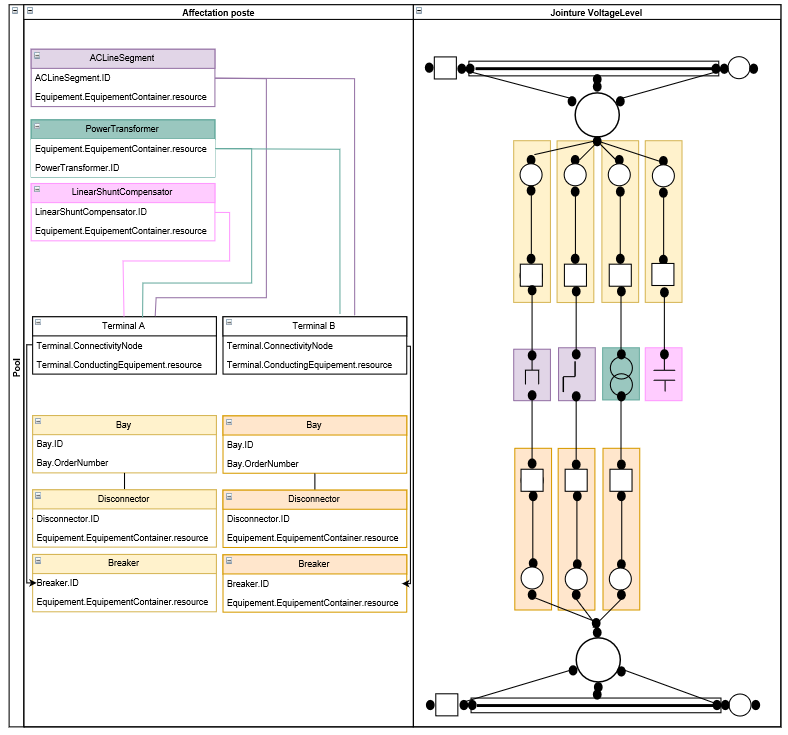
\includegraphics[width=0.475\textwidth]{0.figuras/Jointure_VoltageLevels.png}}
    \captionof{figure}{\textit{ACLineSegment, PowerTransformers} and \textit{LineShuntCompensator} as linking or terminal elements of  \textit{VoltageLevels} respectively.}
    \label{fig:VoltageLevel-interconnections}}
\end{figure}

\begin{itemize}[label={}]
        \begin{itemize}[label={}]
 Analogically, when \textit{BusbarSection} position ends up on a reactive power tool modifier, whether a compensator or a coil, \textit{LinearShuntCompensator} is deployed. 
 
 \nameref{fig:Terminal-ConnectivityNode} takes good note of all these affirmations and schematic representation of the exemplified post seek to easy the model understanding of the reader.
\end{itemize}
    \end{itemize}
    

\begin{itemize}[label={}]
\begin{itemize}

\item Contrarily, a \textit{Disconnector} will be the \textit{EquipementContainer}\footnote{Whose alpha-numeric attribute will be the same as that of the identifier \textit{Disconnector} in question, named \textit{Disconnector.ID}.} of two different \textit{Terminals}, which will be linked to others through the \textit{Terminal.ConnectivityNode} notion.

\end{itemize}
    \end{itemize}

\subsection{Data management}
\label{sub:AIG:data-management}

These classes are interlinked and played with in FME. Two main stages will encompass the natural activity carried out in the software:
\begin{itemize}
    \item Hierarchic chain enrichment through classes merging.
    \item Graphical properties attribution and object displaying configurations.
\end{itemize}

In a second stage, the approach undertaken has seeked to modularize FME treatments, which quite systematical and rigorous, just will require minimal modifications for several specific cases, as that of the \texttt{PowerTransformer-PowerTransformerEnd} linking steps for example. This processus contributing to alligerate considerably the files size, yet as the schematic complexity.

\subsubsection{FME fonctionalities}
\label{subsub:AIG:data-management:FME-fonct}

First of all, attributes are imported in a vast range of different input formats, many of them neatly in Feature-Type XML Reader form, and thereafter a first methodological filtering will be performed, in case several of them re null or found empty.

EXPLICAR LAS DIFERENTES FUNCIONALIDADES DE FME MAS ANADIR SINOPTICO TRATAMIENTO FME

Y QUE ES EL RESULTADO QUE DAN CADA UNA DE ELLAS

\subsubsubsection{\textit{- AttributeFilter}}

In the first placed, not all attributes are always imported from CIM model, on pursuit of performance boosting and discretional workspacing. This is easily feasible thanks to FME Readers, which regardless of the input format enable attribute selecting.

\subsubsubsection{\textit{- FeatureMerger}}

This tool is the most important attribute management operation towards an UML hierarchical para-model creation, which, should be kept in mind, is one of the major contributions of the work undergone towards a solid and robust database patrimony creation. Theoretically speaking, it consists of a mechanism for cross list joining, which related on several \textit{pivotting} arguments.Two list input types enter a \textit{FeatureMerger} on principle: 
\begin{itemize}
    \item \textit{Requestor} will add the main list, that is all the arguments (which will be completely kept unless otherwise specified) remain on the output merged list
    \item \textit{Supplier} will furnish the \textit{Requestor} with as many as \textit{pivotting} arguments stipulated.
\end{itemize}

However, multiple options configuration are available on FME FeatureMerger toolkit, and list are obviously transposable, so are their arguments and pivotal arguments.

\subsubsubsection{\textit{- SubStringExtractor-StringConcatenator}}

Shall be kept in mind that we are continuously working with alpha-numeric chains of characters, which sometimes requires from a thorough, yet symptomatic attribute tailoring. In particular, \textit{pivot} list attributes were systematically prefixed by a #, which shall be taken into account it a consequent pivotal coherence had to be kept among differnet lists. 

\subsubsubsection{\textit{- TestFilter-Sorter}}

Parametric filtering being necessary at times, Test Filtering and List sorting tools resulted to be extremely important to this extent, as coherence could be easily lost otherwise.

For instance, when discerning between breakers positions on top or underneath a post, attribute \textit{Bay.bayOrientation} was studied. Different values of this attributes required different treatments and so that different representation criterias, as shown in \nameref{subsub:AIG:diagram-layout:object-picto-properties} section maxims. It is in this spirit that attribute filtering and sorting may be used for conditions statement and consequent processes divergences introduction.

\subsubsubsection{\textit{- ListBuilder-ListSorter}}

Following the statement up here, elements grouping through list is also extremely important for parametric treatment. Common-sourced elements may be managed equally, and so this feature enables this possibility. On top of that, list can afterwards exploited, there retrieving the same continent structure than before its building.

\subsubsubsection{\textit{- CoordinateExtractor}}

Some elements have intrinsic geometrical properties, which are assigned to them by FME geometrical toolkit creator possibilities such as VertexCreator among others. When extraction of this properties needed, this tool enables its acquaintance for posterior designing or redrafting.

\subsubsubsection{\textit{- VertexCreator}}

The geometric creator by excellence, it enables any 2D geometry (Point, Line, Polygon, etc) creation and has been extensibely used along the treatment because of its simplicity and easy debugging properties.

\subsubsubsection{\textit{- PointConnector}}

Once points created, sometimes is interesting its line-linking according to several properties. This is the case, for example, of \textit{BusbarSection} creation or \textit{Disconnector-Breaker} joining. PointConnector enables all this and other possibilities, providing that elements are well sorted and structured.

\subsubsubsection{\textit{- LineJoiner}}

One step furtuer from PointConnector onto element joining is LineJoiner. That is, once the line created through PointConnector or VertexCreator implementation, they can be likewise linked between them parametrically.

All this toolkit internalized, its deployment can be broadly split on 3 main stages: 
\begin{itemize}
    \item \textbf{Attribute importing and list systematical enrichment}, provoking the whole hierarchical chain slub.
    \item \textbf{Filtering and discernible treatment}, for posterior parametric representation or eventual treatment processes set up.
    \item \textbf{Single-post Diagram layout displaying} according to the metadata nature, with their corespondent \textit{ACLineSegment} linking inter-post lines.
\end{itemize}

That is, through list merging, attributes are incorporated to their UML model, showing functional dependencies between classes off.

When necessary, certain exceptional treatment are implemented, always keeping a systematical rigorous approach. 

Depending on nature and parametric properties, different displaying are performed, by different pictographcial properties affectation

Whole process can be found on \nameref{Acronyms} chapter. NANDIR TODO EL ESQUEMA UNA VZ TERMINADO ( AQUI SOLO MOSTRARLO POR PARTES)

EXPLICAR PROCEDIMIENTO PASO A PASO INTRODUCIENDO A CADA VEZ LOS ESQUEMAS PARCIALES DE CONEXION DE CLASES - ATRIBUTOS??

GRAN ESQUEMA DE CONEXION DE LAS CLASES CON ARGUMENTOS CLAVE Y PROCEDIMIENTO PASO A PASO

\subsection{Diagram layout drawing}
\label{sub:AIG:diagram-layout}
Once the different classes levelled and their bounding hierarchical links identified, the time to attribute functional dependencies and implement their diagram layout, in a first stage in a post separated format followed by an integrating procedure, plus a space-optimization seeking. As the step between \autoref{fig:CIM_diagram-layout-skeleton} and \autoref{fig:CIM_diagram-layout} shows, every class notion correspond to an electric element, whose representation form is standardized and spread following \autoref{subsub:AIG:normative:elec-representation} specifications, which will be deeply tackled in detail in the following section \ref{subsub:AIG:diagram-layout:non-eq-notion}. 

All those elements will not be unconditionally represented on the pursuit of cache memory optimization\footnote{And specially taking into account that Herge's team-lead is finally seeking to exploit its layout in a tablet format, which will compromise even more strongly display featuring.}, but may remain in the skeleton architecture reproduction. In this way, we will perform a conditional displaying as we zoom out or in throughout the SRC and SNC schemes under the condition that no more than 10 000 objects per screen will ever be represented, with a seeked optimal number of about 8 000. 

\subsubsection{Non-equivoque notion}
\label{subsub:AIG:diagram-layout:non-eq-notion}

It is certainly important when transposing the structure to the drawing to rigorously represent every element for a non-equivoque layout of the on-field electrical structuring. In other words, each element unity shall remain unchanged all the treatment long, regardless of the enrichment process it may undergone. 

For separate unit components representation and posterior assembling, it is primordial to keep these notions unaltered in seek of a two-sided bijectional relation between databases and diagram layout representation.

Additionally, all these model solidity maxims could be implemented through \textit{DupplicateFilter} FME toolbox functionality. called , which keeps just one unique element per identifier.

NAME SUBSPACES AND PHOTO OF BIJECTIONAL SPACES RELATION THEN USE SAME NOTATION FOR APPARTAT HEREAFTER

\subsubsection{Object unalterepictographic properties attribution}

\label{subsub:AIG:diagram-layout:object-picto- properties}

Position plus, altogether with the pictographic icon, discussed in \nameref{sec:approach:software:ArcGIS} section aofterwards, will be the two main properties to assign to an element. Therefore, position will be created by the operation of two coordinated systems: the local one of the intrapost himself \(\lbrack \mathscr{X}_{local}, \mathscr{Y}_{local}  \rbrack \), and that of the macro post position inside the whole representation scheme, e.g. \(\lbrack \mathscr{X}_{origen puesto},{Y}_{origen puesto} \rbrack \), who will be the one to optimize on \nameref{subsub:AIG:SLV:graph_theory} subsection.

Devices will be systematically positioned in accordance to, in first, the fonctional dependencies with another objets, plus their given attributes as \textit{Classes} (\texttt{Bay.Bayorientation}, and \textit{SCADA step} neatly, as shown \hyperref[fig:post_draft]{hereafter}).

\begin{figure}[h]
    \centering
    \parbox[t]{1\textwidth}{
    {\centering
    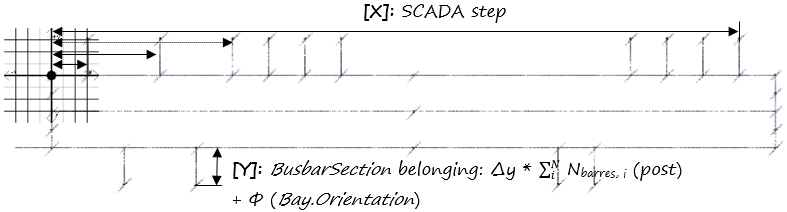
\includegraphics[width=1\textwidth]{0.figuras/Draft-post-represenation.png}}
    \captionof{figure}{\textit{Saint-Valentin} (\texttt{SSV.O-P71}) post first FME representation draft, with its local coordinates position parametric model.}
    \label{fig:post_draft}}
\end{figure}

Thus, the subspace general coordinates \(\lbrack \mathfrak{X}_{general}, \mathfrak{Y}_{general} \rbrack \) of a certain element, contained within a post, will be expressed as the linear combination\footnote{for easying elements magnitude in contrast with post gapping.} of \(\lbrack \mathscr{X}_{origen puesto},{Y}_{origen puesto} \rbrack \) and \(\lbrack \mathscr{X}_{local}, \mathscr{Y}_{local}  \rbrack \) subspaces:
\\


\begin{equation}  \left\lbrace
\begin{array}{cc}
     & {\mathfrak{X}_{general}}=\mathscr{X}_{Post origin}+\mathscr{X}_{local}  \\
     & {\mathfrak{Y}_{general}}=\mathscr{Y}_{Post origin}+\mathscr{Y}_{local}
     \end{array}
     \right.
    \end{equation} 

Being the post coordinates fixed as in the following, they will be matter of long study in \autoref{subsub:AIG:SLV:graph_theory}:
ling Breaker's 

\begin{itemize}
    \item \(\mathscr{X}_{local}=0 \leftrightarrow\mathfrak {X}_{general}=\mathscr{X}_{Post origin}, \) placed on the left-sided Coupling Breaker's x-axis. 
    \item \(\mathscr{Y}_{local}=0 \leftrightarrow\mathfrak {Y}_{general}= \mathscr{Y}_{Post origin}, \) placed on the first BusbarSection's y-axis.

\end{itemize}
From the post introspective PoV, objects local positioning \(\lbrack \mathscr{X}_{local}, \mathscr{Y}_{local}  \rbrack \)  must be systematically parametrized in a rigorous way so that every element positioning is completely unique and faithful, his fundamentals raising no doubts about which criteria was approached for it. 

In this purpose, and once post position local origin establishedon the first bar at the coupling elements-high, as shown in \autoref{fig:post_draft}, objects coordinates will be referred to this origin. To this effect, the main variables which will be used to parametrize those positions in the following are:

\begin{itemize}[label={-}]
\item \texttt{Bay.bayOrientation}
\item \textit{SCADA step} \footnote{In DPC\textsuperscript{2} files, \textit{Pas} \quad \textit{SCADA} is given in multiples of 10\cite{cahier_dpc2}.}
\end{itemize}
 
Being the position breakers the firsts to be placed, every post elment position will be 2Dimensionally-referenced to this following these rules:

\subsubsubsection{- Breakers}
\begin{equation}
\mathscr{X}_{local}= \frac{SCADA & step}{10}    
\end{equation}

For example, \autoref{fig:post_draft} shows \textit{Saint-Valentin} post behaviour in \textit{Lille}-SRC zone, the \texttt{Bay.bayOrderNumber} argument fixes the horizontal position\footnote{Being the first coupling (if existing) situated on the zero of abscisa axis}, while the \texttt{Bay.orientation}, plus the adherence to a certain bar out of the total number in the post will determine its vertical's:


\( \mathscr{Y}_{local}=231321\) will be generatlly formulled as \( amfjaf\), which finally will declinate, in fonction if \textit{Bay.bayOrientation} vaule is \(\mathsf{H}\) (up) or \(\mathsf{B}\) (down) onto:

\begin{equation}  
\mathscr{Y}_{local}=\left\lbrace
\begin{array}{llllll}
     & \textit{Bay.bayOrientation} & =\(\mathsf{H}\) &\Longrightarrow &\mathscr{Y}_{local}^{up}=1 \\
     &  \textit{Bay.bayOrientation} & =\(\mathsf{B}\) &\Longrightarrow & \mathscr{Y}_{local}^{down}=\sum_{n=1}^{\ N_{bars}^{max}} (1-n) * \Delta y^{SA}  & \forall n \in \mathbb{N}
     \end{array}
     \right.
    \end{equation} 

\subsubsubsection{- Coupling breakers}

Coupling breakers are normally place at the beginning or in the end of the bar, which is already taken into account in their \textit{SCADA step} parametric initialization. Anyway, this last will be subsequently verified for every of these elements in line with the following equations:
\\
\begin{equation}
    \mathscr{X}_{coupl. breaker}=\left\lbrace
\begin{array}{llllllll}
     & \textit{Bay.bayOrderNumber} & =\(\mathsf{0 - Left}\) &\Longrightarrow &\mathscr{X}_{coupl. breaker}^{left}=0 \\
     & \textit{Bay.bayOrderNumber} & \neq\(\mathsf{0 - Right\footnote{max_i(X_positions(poste i))}}\) &\Longrightarrow &\mathscr{X}_{coupl. breaker}^{right}=max (\mathscr{X}_{positions}) & \forall n \in \mathbb{N}
     \end{array}
     \right.
\end{equation}

\subsubsubsection{- Bars}

Bars are drawn as lines by aggregating in X the different positions linked to the correpsondent \texttt{BusbarSection}-linked ouptut positions, whereas Y position will depend on a counter of \texttt{BusbarSections} belonging to the \texttt{VoltageLevel} in question.

For the abscis coordinate, they are thereafter drawn in fonction of the maximum and minium (\( \mathscr{X}_{local}^{max}\) to \( \mathscr{X}_{local}^{min}\)) positions of the bar to whom the devices belong.

\begin{equation}
    aa
\end{equation}


Decoupage barre en BTS
Positionnement celllules BTS
Elementos diferentes e independientes



\subsection{Problems faced}

Several unexpectted problems have been encountered as project advanced, being all of them presented herafter. In addition, the wy they were identified, tackled then solved is exhaustively explained, being the \textit{modus operandi} itself more interesting thatn the final output of it ijn most cases.

The methodology followed to achieve the objectives is shown in Figure
1.3. As can be seen, this work consist of ve main tasks, organized in several
chapters.
Chapter 2 deals with the literature survey of current strategies to optimize
engine efficiency. In this sense, a comprehensive review is performed
to understand the engine research background over the last 2 decades. The
trade-o between emissions and eciency, along with the potential of thermal
balance for engine evaluation is discussed in this chapter. An extensive amount
of works dealing with RICE thermal balances is used for the discussion, where
the importance of establishing a comprehensive methodology for its analysis
is evidenced.
Chapter 3 shows a complete description of the experimental installations
and the reference thermodynamic model, including:
 Details of the instrumentation required to perform the experimental
work.
 A description of the dierent sub-models included in CALMEC and SiCiclo
(0D thermodynamic tools), detailing which of them need to be further
upgraded as done in the following sections.
Based on the experimental and modelled information available, Chap-
ter 4 introduces an integral experimental and modelling methodology to perform
the thermal balance, called Global Energy Balance (GEB). This methodology
considers 2 main points of view, on the one hand the External GEB,
which considers the engine as a black box and whose terms are obtained mainly
through experimental techniques; and on the other hand the Internal GEB,
which takes into account all the internal energy degradation phenomena due
to thermal and mechanical processes (e.g. heat rejection and friction). For the
sake of completeness, the relationship between internal, and internal-external
terms will be also detailed in this chapter. Special analysis of some heat rejection
terms used for the calibration and validation stages will be provided,
along with an experimental uncertainty analysis.
Taking into account the description of the energy terms provided in
Chapter 4, the improvement of some reference sub-models and the proposal 
of new ones will be necessary. Therefore, Chapter 5 is dedicated to the
development and validation of specic heat transfer and mechanical losses
sub-models, along with a comprehensive uncertainties adjustment process.
To asses the potential of the methodology developed in this work, Chap-
ter 6 describes the use of the GEB in two dierent engines: one conventional
1.4 Methodology 9
multi-cylinder 4-stroke Diesel engine, and a research single-cylinder engine.
The work presented in this section is divided in 2 steps:
1. Description of the sub-models calibration methodology based on the
equivalent heat transfer terms presented in Chapter 4, along with the
uncertainties tuning described in Chapter 5.
2. Performing the GEB analysis in some parametric variations, aimed at
the integral energy characterization of the studied engines, along with an
example of the use of the calibrated sub-models and GEB for predictive
applications (using a 0D thermodynamic model).
Finally, Chapter 7 summarises the work performed and shows the main
conclusions regarding its contributions. In addition, some proposals for future
works are lastly discussed.
For convenience, besides each chapter bibliography, at the end of this
document all the references cited are organized in alphabetic order, indicating
the pages where they are cited.

ANADIR QUIZA UNA TABLA DICIENDO LOS DIFERENTES PROBLEMAS IDENTFICAIDOS + COMO HAN ISDO ABORDADOS A NIVEL TECNICO( AUE DIFICULTADES ADICIONALES PODRIAN DECRIVARSE DE EZTO) Y CUAL HA SIDO LA SOLUCION FINAL IMPLEMENTADA

Several problems have been encountered when layout diagram representation
\subsubsection{LITs crossing}

Due to the massive amount of post to represent, apart from  the objective divergence between concomitant projects in the matter, we finally were encountered with a multiple \textit{ACLineSegment} crossings, being the post origin position the root of the problem

Three-linked at a time post were triangulated, its circle identified and set in common for the three of the them

ANADIR FOTO ANTES DESPUES

\subsection{Technical issues}
\label{subsub:AIG:technical-issues}

Constituting the graphical interface for the most part of Rte's on-field business users, an important flux of financial actives depend on Herge's fate, which makes it a substantially constrained project in terms of users necessities. They are the ones who grab the major part of the negotiating power and therefore encompassing the trail of the project.

Consequently, the results of the displayed methodology shall remain certainly close to the actuals, and changes may be considerably evident, flexible and easily apprehensible. This incertitude reigning all the project long has deeply impacted its approach and methodology, always on the pursuit of flexibility by means of modularity and adaptability possibilities in connection to the future additional steps Herge could take, yet as all its impacted partners.

In keeping with the aforementioned maxim, an additional difficulty pop up: notably, several technical issues have been accordingly identified throughout the complete project, whom could be systematically approached and dealt with, a well-focus approach beforehand has disminuiss their imapct and let to identify most of them in advance.

In this concept, FME treatments have been performed the most modularized possible, through the use of versionable \textit{Customer Transofmers}, which could be update to each upgrading or modification of the treatment "alpha". Once its use exhausted, ArcGIS tools were maximally developed and in the most logical way, using the \textit{Network Analyst} toolpackage first and foremost, as it was the one that most approached our technical needs.

Specifically, two main difficulties encompassed the unexpected problematics abborded: 

\begin{itemize}
    \item First of all, crossing-lines between post problems were appreciated, specially when charging big areas of study\footnote{Which seems completely normal, taking into account the electrical network is finally a growing mesh, for ensuring a good clients level of service, plus flexibility in maintenance and exploitation.} 
    \item The second problematic refers to several problems occurred regarding post problems management at each iterative step on ArcGIS, which compelled to objects overlapping fixing, ended sometimes on recurrent overlapping. This was due to a non-adequate post position changes awareness, blocking graphs algorithm from taking into account the new situation of the modified post-positions-matrix.  
    \end{itemize}

Anyway, these problems have been correctly addressed and finally solved, as shown in \hyperref[susub:AIG:technical-issues:postpositionmanagement]{the following subsection}, for attaining functional \nameref{sub:AIG:technical-issues:proposed-solutions}. Altogether with a good technical documentation of the chosen decisions, the extra effort linked to the previously stated will enable to lighten future actions during the subsequent versions of Herge.

\subsubsection{Recurrent post position management acknowledgement}
\label{subsub:AIG:technical-issues:postpositionmanagmement}

As previously stated, if we are seeking to automatize the post position in a recurrent basis, there must be a way of acknowledging which approach have been performed plus reloop those position in the canonical algorithms. 

\subsection{Proposed solutions}
\label{sub:AIG:technical-issues:proposed-solutions}

 Envisablable solutions have been strivedfrom an ArcGis basis, on which \textit{Network Analysis} tools enabled automatic management of post position, building on a Graph theory theoretical background.
 
\section{Layout optimization}
\label{sec:AIG:layout_optimization}

The last stage of the work undertaken was to be able to manage post position so that the whole layout may be optimized. A double slope opens  both theoretically and practically.

This way, from one hand a theoretical background documentation has been proceeded of a correct industrialized state of art conscience raising. 

\subsection{Principe}

The intersection of different methodological techniques have enabled the open up of a logical implementation of post position optimization.

\subsection{Theoretical background}
\label{sub:AIG:SLV:theoretical background}

As underlied in the section \ref{sub:AIG:normative}, no industrialized documentation and complete lack of framework has been stated on most of the techniques implemented through this work. Their avnant-garde statusli and strictly research-scope character prevents its technical transportation from already undertaken on corporate projects. There lays also the interest of this study ,as recurrently ennounced.

\subsubsection{Graph theory}
\label{subsub:AIG:SLV:graph_theory}

Well-spread on the treatment of geodatabase information exchange, graph theory has been extensively developed in the end of 80s, and 90s. This process us consisting on relative weight assignation of different resources, lets correlative solution layout optimization, its exploitation o n electrical diagrams optimization remains notably unexploited.

Force-based network representation as that of \hyperref[fig:force-diagram]{the following diagram}

\begin{figure}[h]
    \centering
    \parbox[t]{1\textwidth}{
    {\centering
    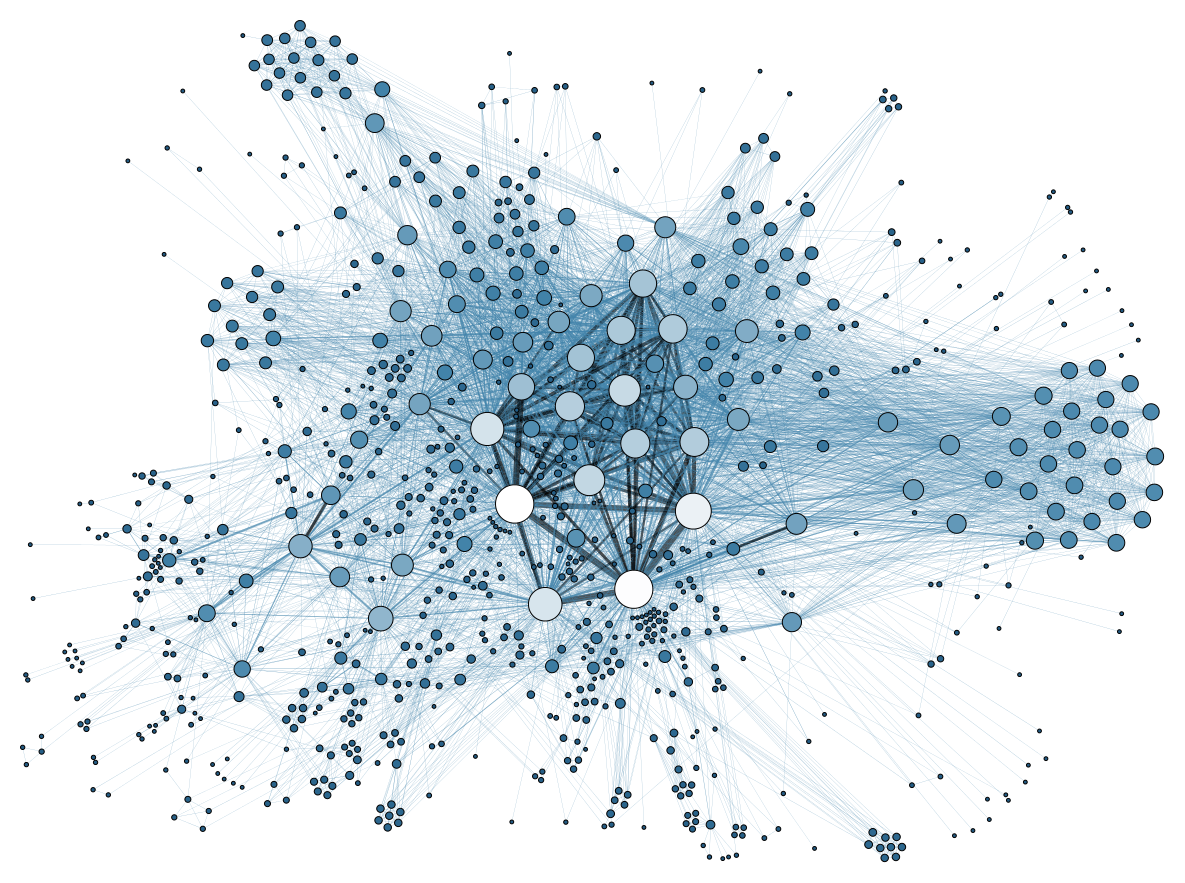
\includegraphics[width=1\textwidth]{0.figuras/Social_Network_Analysis_Visualization.png}}
    \captionof{figure}{Force diagram assessment performed on a social network analyst visualization.(\href{https://en.wikipedia.org/wiki/Graph_drawing}{Wikipedia-sourced})} 
    \label{fig:force-diagram}}
\end{figure}

\subsubsection{Metaheuristic algorithms}
\label{subsub:AIG:SLV:graph_theory:meta_algorithms}

On the pursuit of automatizing data dumping, yet as characterisitical cases treatment, several methaheuristic algorithms have been systematically introduced. Their functioning basis remain on the principle of anomalies creation, plus their propagation thought the hierarchical chain, serving to create unthinkable situations. Those anomalies will not get reproduced anymore as it happens, for instance, in the evolution chain theory of Lamarck, the one on whom the Metaheuristic algorithms relay.

\subsubsection{Voronoi diagrams}
\label{subsub:AIG:SLV:Voronoi}

In mathematics, a Voronoi diagram is a partitioning of a plane into regions based on distance to points beforehand specified in a certain subset of the plane. Through Delaunay triangulation of a set of points is dual to its . 

\begin{figure}[h]
    \centering
    \parbox[t]{0.7\textwidth}{
    {\centering
    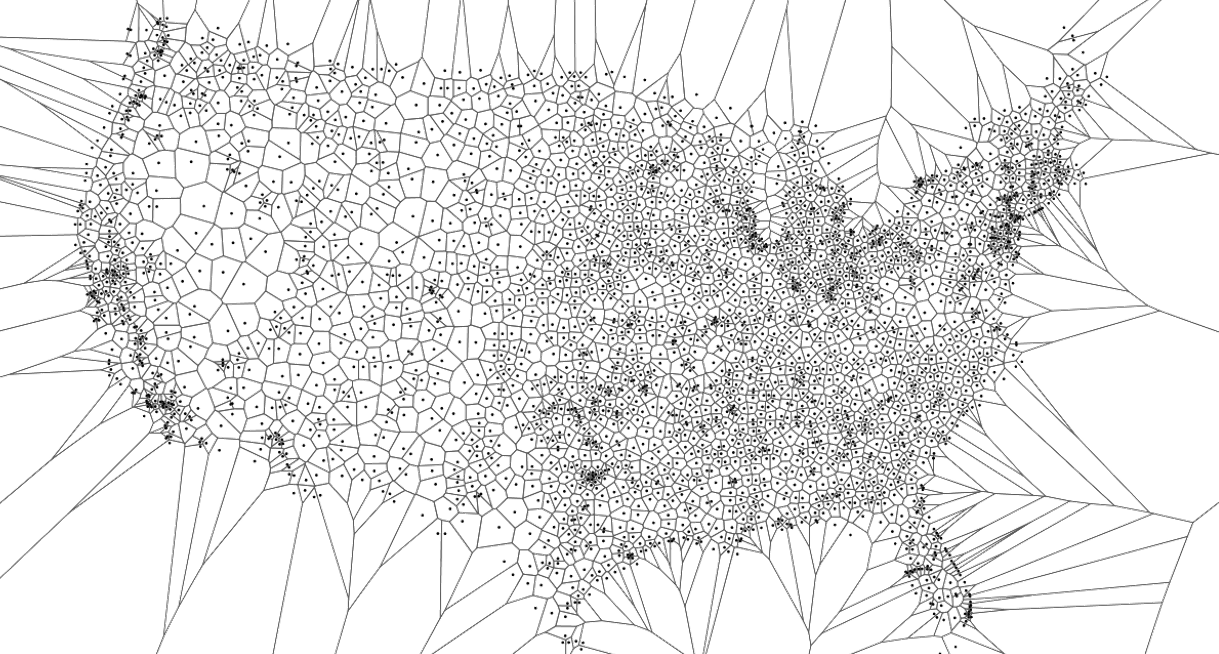
\includegraphics[width=0.7\textwidth]{0.figuras/Usa_airports_voronoi_diagrams.png}}
    \captionof{figure}{Force diagram assessment performed on a social network analyst visualization.(\href{https://en.wikipedia.org/wiki/Voronoi_diagram}{Wikipedia-sourced})} 
    \label{fig:Voronoi-diagram}}
\end{figure}

To our case of study, they let to characterize the relational dependencies implementation of relational databases. And what is more important, its application was already integrated in FME toolkit, what lighten notably up its implementation and supposed no derives regarding the previous approach.

In geometry, Voronoi diagrams can be used to find the largest empty circle amid a set of points, and in an enclosing polygon; e.g. to build a new supermarket as far as possible from all the existing ones, lying in a certain city.
Voronoi diagrams together with farthest-point Voronoi diagrams are used for efficient algorithms to compute the roundness of a set of points. The Voronoi approach is also put to good use in the evaluation of circularity/roundness while assessing the dataset from a coordinate-measuring machine.
Modern computational geometry has provided efficient algorithms for constructing Voronoi diagrams, and has allowed them to be used in mesh generation, point location, cluster analysis, machining plans and many other computational tasks.


\subsubsection{MDS}
\label{subsub:AIG:SLV:MDS}

Multidimensional scaling (MDS) 

\subsection{Practical solutions}

Once enough theoretically formed, their implemetnation on the \nameref{sec:approach:software} deployment has supposed several challenges, and therefore introduced new milestones in a development approach.

\subsubsection{Maching learning}
\label{sub:AIG:machine_learning}

Well-spread in the latter years, machine learning enables data scientists to systematically acknowledge intelligently classified situations, and therefore perform systematical algorithms in concordance.

\subsubsection{ArcGIS optimization tools}

GIS tools are deeply exploited in cartography and geographical decisions taking assessment processes. 

Regarding our case of study, its toolkit, and notably \textit{Network Analyst} functionality enabled the different post position acknowledgement, plus their management in order to a more intelligent space optimization.

\subsubsubsection{Network Analyst}

This ArcGIS extension functionalities range are apparently inexhaustive regarding geodatabase intelligent management processes, e.g behaviour predicting, meshes of any nature analyzing, among others.

Traditional questions in geographical optimization such as shortest-path finding, business optimal geoexpansion, 5-minutes zone regrouping or the notably famous paradigm of the\textit{Seven Bridges of Königsberg} are easily answered on GIS software. 

Network Analyst fundamental algorithms help assessing this kind of questions and others. Regarding the subject ofour study, a certain network mesh, formed by different post positions, plus the linking lines among them, was presented. The aim was to subsequently optimize these positions in seek of minimizing LITs length and crossing with others. 

This algorithms seemed to respond quite accurately to the presented needs, additionally contributing with unknown fucntionalities that certainly enriched the whole intelligent procedure.
% -------------------------------------



	


% ---------------------------------------------------------------------
% ---------------------------------------------------------------------
% ---------------------------------------------------------------------
% Fin


\chapter{Outputs and results}
\label{cap:AIG:Outputs}
\begin{Resumen}

This first chapter aims on giving the reader a panoramic overview of the problematic of study, raising consciousness not only on the work carried out but on a more introspective PoV of its day-to-day approach, yet its working atmosphere. Thus, the \nameref{sec:Intro:thesis-purpose} is firstly stated, altogether with a \nameref{sec:intro:background} and a work-frame environment within \nameref{sec:Intro:HERGE}\footnote{Projet HERGE was the teamwork in which my \ingles{stage} was framed, will be explained in detail in the section \ref{sec:Intro:HERGE}} brief inductions, technically enriched on  \nameref{sec:intro:software} section.  

\end{Resumen}
\PartialToc
% ---------------------------------------------------------------------
% ---------------------------------------------------------------------


\bigskip
\lettrine[lines=2]{\textbf{S}}{}hall be kept in mind that the final objective of the undergone work was to end up with a logical, representative layout of the corporate electrical network in HV and super HV. In the following, several livrables of the work pursued will be presented, in order to shed more light on the validity of the work undergone, sustaining its methodology and approaching.

In addition, a path guide of the steps undergone to reach the final solution is performed, for the reader to more logically  understand the decisions taken, and the improvements introduced. 

\section{Overview}

In a first approach, the different element typologies have been represented gradually, by affecting them incrementally the iconographic properties for correctly retaken the UML structuring, plus the conventional properties following the \nameref{subsub:AIG:normative:elec-representation}.

In this way, the functional schemes will be step by step complemented with the introduction of every \textit{Class} notion.

Once the functional structure retaken in FME as explained in the \nameref{subsub:AIG:diagram-layout:object-picto- properties} subsection, position looped assessment in ArcGIS will modify the post positions gradually.

\section{Utilization}

Conversely, several objectives have been introduced following users expectancy, and therefore several applicability have been introduced on that point.

In a future extent, a gateway for managing the position of every element and adhere to each of them the pictographical properties as conceived in the actual interface, so that users are not impacted on the whole scheme display. Nonetheless, the complete hierarchical scheme will be automatically reproduced, so that every modification could be exploited to the totality of the diagram, making new posts aggregation much more logical and work-demanding.

\subsection{Users}

The most controversial point was the staticity of users, regarding Herge capabilities and features. Taht is, after been already used to a static, clear and functional (yet not optimal, as daily anomalies were identified) portal, users seemed skeptical to any change, and the complete automatizing of Herge's schemes will comport a major one.

Taking into account that most of on-field operations were traditionally performed on the basis of Herge schemes, the risk undertaken of a non-performing comprehension of a topology due to changing pictographs was substantially high.

\subsection{Industrialization process}

Firstly fed on RDF databases, exchanges with StanWay lead to the providing of structured XML files, deeply transformed through several databases feeding and metadating operations.

Several steps embarked the complete schema reproduction. Its different parts where systematically added, by following a continuous logic. Hence, each element kind was added at a pase, completing the schema systematically. The elements classification can be found in the section regarding \nameref{cap:AIG:diagram:FME} treatment.

It is therefore this treatement which have embarked the majority of evolution regarding industrialization. Its files occuping more than """ KB and their aspect as shown in the figure hereafter, their modularization in the lattest phases of ist implementation, plus the introduction of a GIT for version controlling has boosted its industrialization possibilities, yet as its clarity and retaking facility.

IMAGENES DEL TRATAMIENTO FME ANTES Y DESPUES DE LA MODULARIZACION

\subsubsection{HERGE V2}

At a second stage, and after a proper object projection and interconnection, its positionning was managed through ORACLE linked bases, who were using in the actual handmade diagram layout confection. ArcGIS toolkit enabled its projection on a Webplayer, as well as the elements position modificiation. 

Images of the diagram layout aspect before and after the implementation of the intelligent algorithm can be found hereafter.

IMAGEN DE ANTES Y DESPUES DE UTILIZAR EL NETWORK ANALYST DE ARCGIS


% -------------------------------------
\begin{figure}[h!]
	\bigskip
	\begin{center}
		\parbox{.45\textwidth}{%
		\href{https://polimedia.upv.es/visor/?id=c73f835e-9387-7643-9473-335796a00932}
			{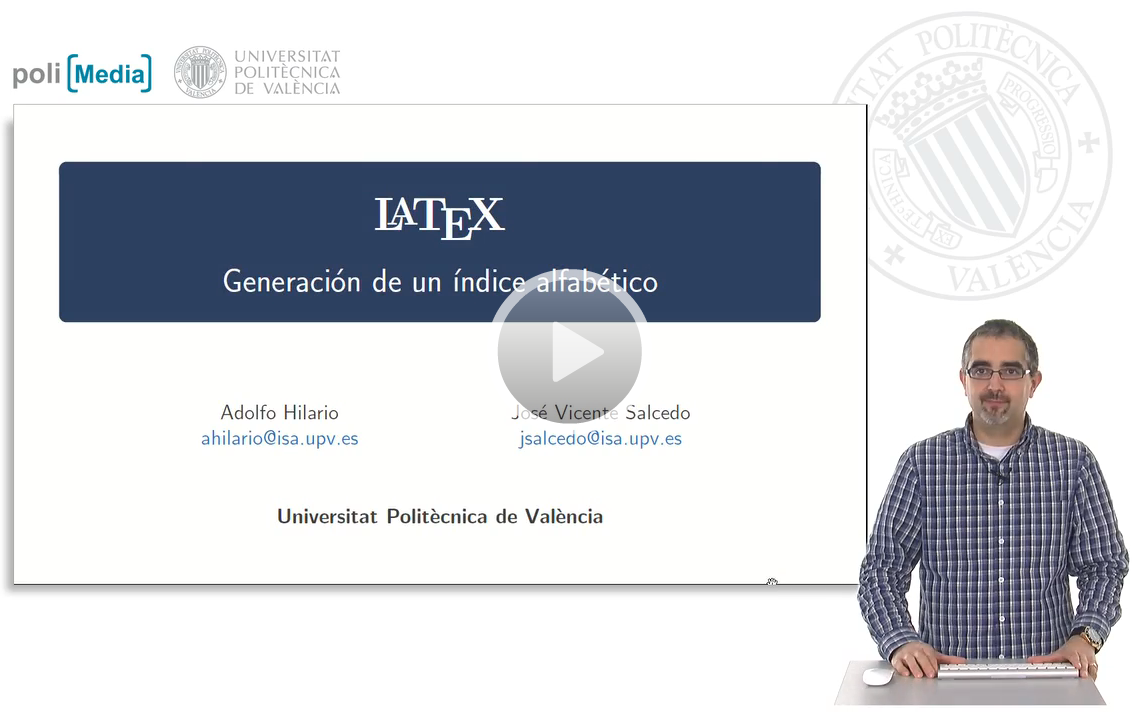
\includegraphics[width = .45\textwidth]{0.figuras/poliMedia_makeindex.png}}}\hfill
		\parbox[t]{.45\textwidth}{\caption{Veo poliMedia: ``Generaci de un ndice alfabico''.
			Haz clic sobre la imagen para acceder al vdeo}
			\label{fig:makeindex}} 
	\end{center}
\end{figure}
\section{Improvement lines}

HABLAR CON HENG ASI COMO CON GERMAN PARA PODER METER TODO ESTO EN COHERENCIA CON LAS MODIFICAICIONES QUE ESTAN HACIENDO AHORA MISMO 

\section{Constraints}

VER LAS REPERCUSIONES QUE EL SEGUIR UTILIZANDO LA BASE DE AUTOCAD PODRIA TENER EN EL FUTURO DESARROLLO DEL PROGRAMA

\subsubsection{Technical constraints}
\subsubsection{Financial constraints}
\subsubsection{Time constraints}
\subsubsection{Usage constraints}


\chapter[Conclusions and future works]{Conclusion and future works}
\label{cap:Conclusion}
\begin{Resumen}
Hereafter, the main conclusions and contributions of this work are stated, altogether with a long term scope of the eventual future works that this work may have on several branches of studies impacted, so far as the studies carried out thereafter.
\end{Resumen}
\PartialToc
\section{Conclusion}
\label{Conclusion:Conclusion}

Objectifs reachment?

\section{Contribution}

\subsection{Industrial use}
\label{sec:manual:matematicas}

\section{Areas of improvement}
\label{sec:manual:hyperref}

Multiple exploitation paths and utilities stand before HERGE, though still several adjustments may be done and overall the others departments compromise is due to its complete adoption.



\begin{minipage}{\textwidth}
	\begin{verbatim}
    \colorlet{colorEnlace}{black} 
	
	\usepackage[
	    {colorlinks},
	    {linkcolor=colorEnlace},
	    {citecolor=colorEnlace},
	    {urlcolor=colorEnlace},
	    {bookmarksnumbered},
	    {breaklinks},
	    ]{hyperref}
	\end{verbatim}
\end{minipage}

\medskip

% ---------------------------------------------------------------------




\LaTeX\ 
\verb'\documentclass[tfg, rm, nomathskip, castellano]{tfgtfmetsii}'

% ---------------------------------------------------------------------

\begin{minipage}{\textwidth}
	\begin{verbatim}
	\usepackage{siunitx}

	\ifenglish
	    \sisetup{output-decimal-marker={.}}
	\else
	    \sisetup{output-decimal-marker={,}}
	\fi
	\end{verbatim}
\end{minipage}


\verb'G = \SI{6.6742(10)e-11}{\newton\square\metre\per\square\kilogram}'\\[1ex]
$G = \SI{6.6742(10)e-11}{\newton\square\metre\per\square\kilogram}$

\verb'c = \SI{299792458}{\meter\per\second}'\\[1ex]
$c = \SI{299792458}{\meter\per\second}$

\verb'\SI{15}{\percent}'\\[1ex]
$\SI{15}{\percent}$

\verb'\num{34572.346e3}'\\[1ex]
$\num{3.346e3}$

La descripci completa del paquete la encontrar en:

{\small\url{http://osl.ugr.es/CTAN/macros/latex/contrib/siunitx/siunitx.pdf}}

\verb'\SI{300}{\EURO}'\\[1ex]
$\SI{300}{\EURO}$




% ---------------------------------------------------------------------
% ---------------------------------------------------------------------
\subsection{Future works}
\label{Conclusion:Future works}
Quitar esta seccion ??

\section{Personal and professional impact of the internship}
\label{sec:manual:impact}

Quitar "of the internship???" del titulo

Porque continuar o no en Rte

Estos son los pasos que debes seguir para \index{Manual de la plantilla!Empezar un nuevo proyecto}empezar un proyecto nuevo con la plantilla \linebreak \texttt{tfgtfmetsii.cls}:

\begin{enumerate}

	\item Duplica la carpeta de ejemplo que has descargado.
    \item Abre el fichero `\verb'Documento_maestro.tex'' con tu editor preferido de \LaTeX.
    \item Gudalo con un nuevo nombre.
    \item Conserva los comandos relativos a: capulos, secciones, bibliograf, etc., que puedan serte es en la posterior confeccin de tu documento.
    \item Elige las opciones de la plantilla `\texttt{tfgtfmetsii.cls}' seg tus necesidades, \autoref{sec:manual:opciones}.
        

\end{enumerate}


% ---------------------------------------------------------------------
% ---------------------------------------------------------------------
% ---------------------------------------------------------------------
% Fin


%\input{.....}

%\input{.....}

%\part{Budget}

%\input{presupuesto}


%\input{planos}

% Otras partes

%\part{....}

%\input{.....}


% -------------------------------------------------------
% -------------------------------------------------------
% -------------------------------------------------------
% Bibliograf�a


\bibitemsep = 3ex
\bibhang = 2em


%\printbibliography[heading=bibintoc, title=\bibname, type=misc ]
\printbibheading[heading=bibintoc]

\printbibliography[type=article,heading=subbibintoc,title={Articles}]
\printbibliography[type=book,heading=subbibintoc,title={Rte internal documents}]


%\printbibl\section{}iography[heading=subibintoc, type=article, prenote={Articles}]
%\printbibliography[heading=subibintoc, type=book, prenote={Rte internal documents}]






% -------------------------------------------------------
% �ndice alfab�tico

\cleardoublepage
\phantomsection

\part{Appendix}
\begin{appendices}


\chapter[Diagram layout samples and evolution]{Diagram layout sample}
\label{sec:Appendix:Diagram}
\begin{Resumen}

In this section you will find several samples of what the final results look like. Most of them are confidential and strictedly limited to RTE activities' use.
\end{Resumen}

\PartialToc

\section{Matlab}
\label{subsec:Appendix:Diagram:Matlab}

\subsection{Code}
\label{subsec:Appendix:Diagram:Matlab:code}

\subsection{Results and outputs}
\label{subsec:Appendix:Diagram:Matlab:results}

\begin{figure}[ht]
    \bigskip
    \begin{center}
        \parbox[t]{0.8\textwidth}{
        \href{}
            {
\includegraphics[width=0.8\textwidth]{0.logos/UPV_horitzontal_color.jpg}}
        \captionof{figure}{First Matlab-driven approach of simple post + coupling reproduction}}
        \label{fig:Matlab-prototype}
    \end{center}
\end{figure}

\section{FME}

\begin{figure}[ht]
    \bigskip
    \begin{center}
        \parbox[t]{0.8\textwidth}{
        \href{https://herge-portal.rte-france.com/arcgis/apps/webappviewer/index.html?id=84a7af442f014844b95939ce3c0067a}
            {
\includegraphics[width=0.8\textwidth]{0.logos/UPV_horitzontal_color.jpg}}
        \captionof{figure}{Schema d'écart haut tension - HERGE visualizer}}
        \label{fig:FME scheme}
    \end{center}
\end{figure}

\subsection{Zones regrouping}

\subsection{Lille}

\section{ESRI results}

\section{CIM Desk example}
\label{sec:Diagram:CIMDesk}


\chapter[FME Block diagram scheme]{FME Block diagram scheme}
\label{sec:FME_Block}

\begin{Resumen}

bajkjlamjfajmkfjamfjkamfjklf
\end{Resumen}

\PartialToc

\section{Schema FME}
\subsection{Treatment zones}
\section{Inspectors}
\section{FeatureMerger}
\end{appendices}
\addcontentsline{toc}{chapter}{\indexname}

\printindex

% -------------------------------------------------------
% Fin del documento

\end{document}